\section{Volume enhancement and validation}

 \begin{figure}[H]
  \centering
  \captionsetup{width=.8\linewidth} 
  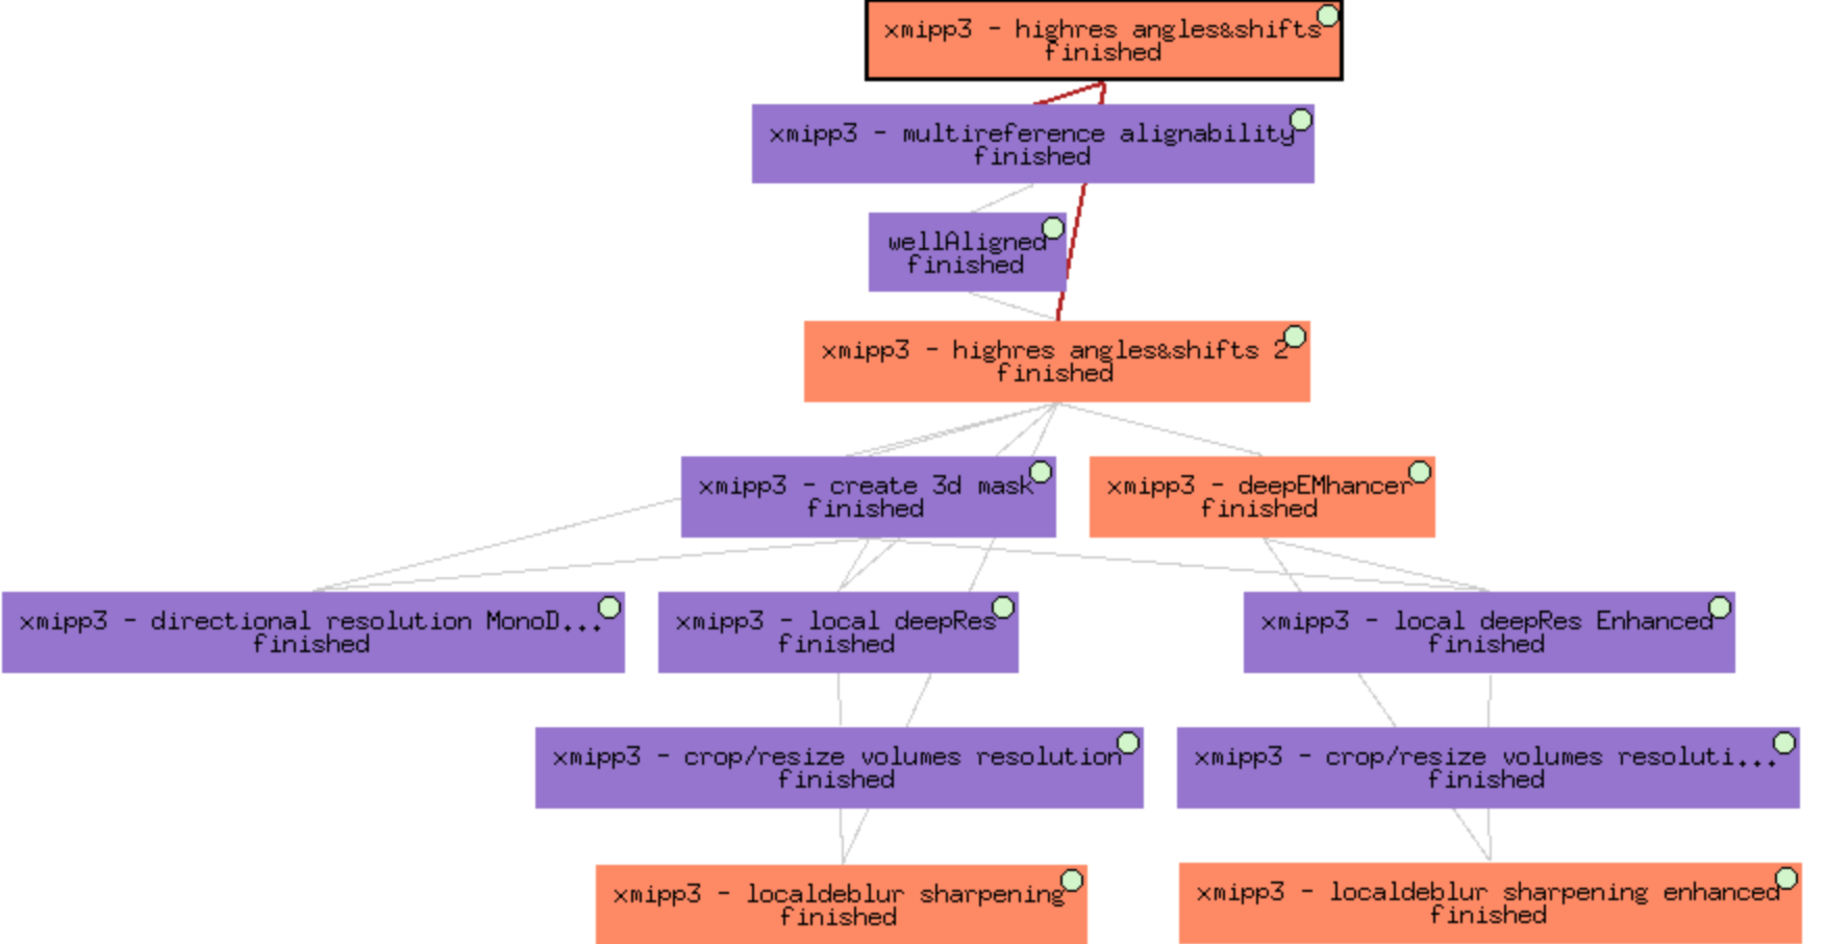
\includegraphics[width=1\textwidth]
  {{images/10_workflow8_Validation_FurtherRec.pdf}}
  \caption{Enhancement and Validation.}
  \label{fig:workflow_7}
  \end{figure}
  
  In this last part of the tutorial, we will verify if what we constructed is reasonable and for this, we have some tests that we can do for this number of particles. The first one,  $Xmipp$ algorithm \ttt{multireference alignability} used in protocol \scommand{xmipp3-multireference alignability} (\ffigure{fig:multireference_alignability}), is going to assess the output map of previous step regarding soft alignability and overfitting of particles and \ttt{3D} map. The input of the protocol requires the map and particles generated in the last refinement step.\\ 

\begin{figure}[H]
  \centering
  \captionsetup{width=.8\linewidth} 
  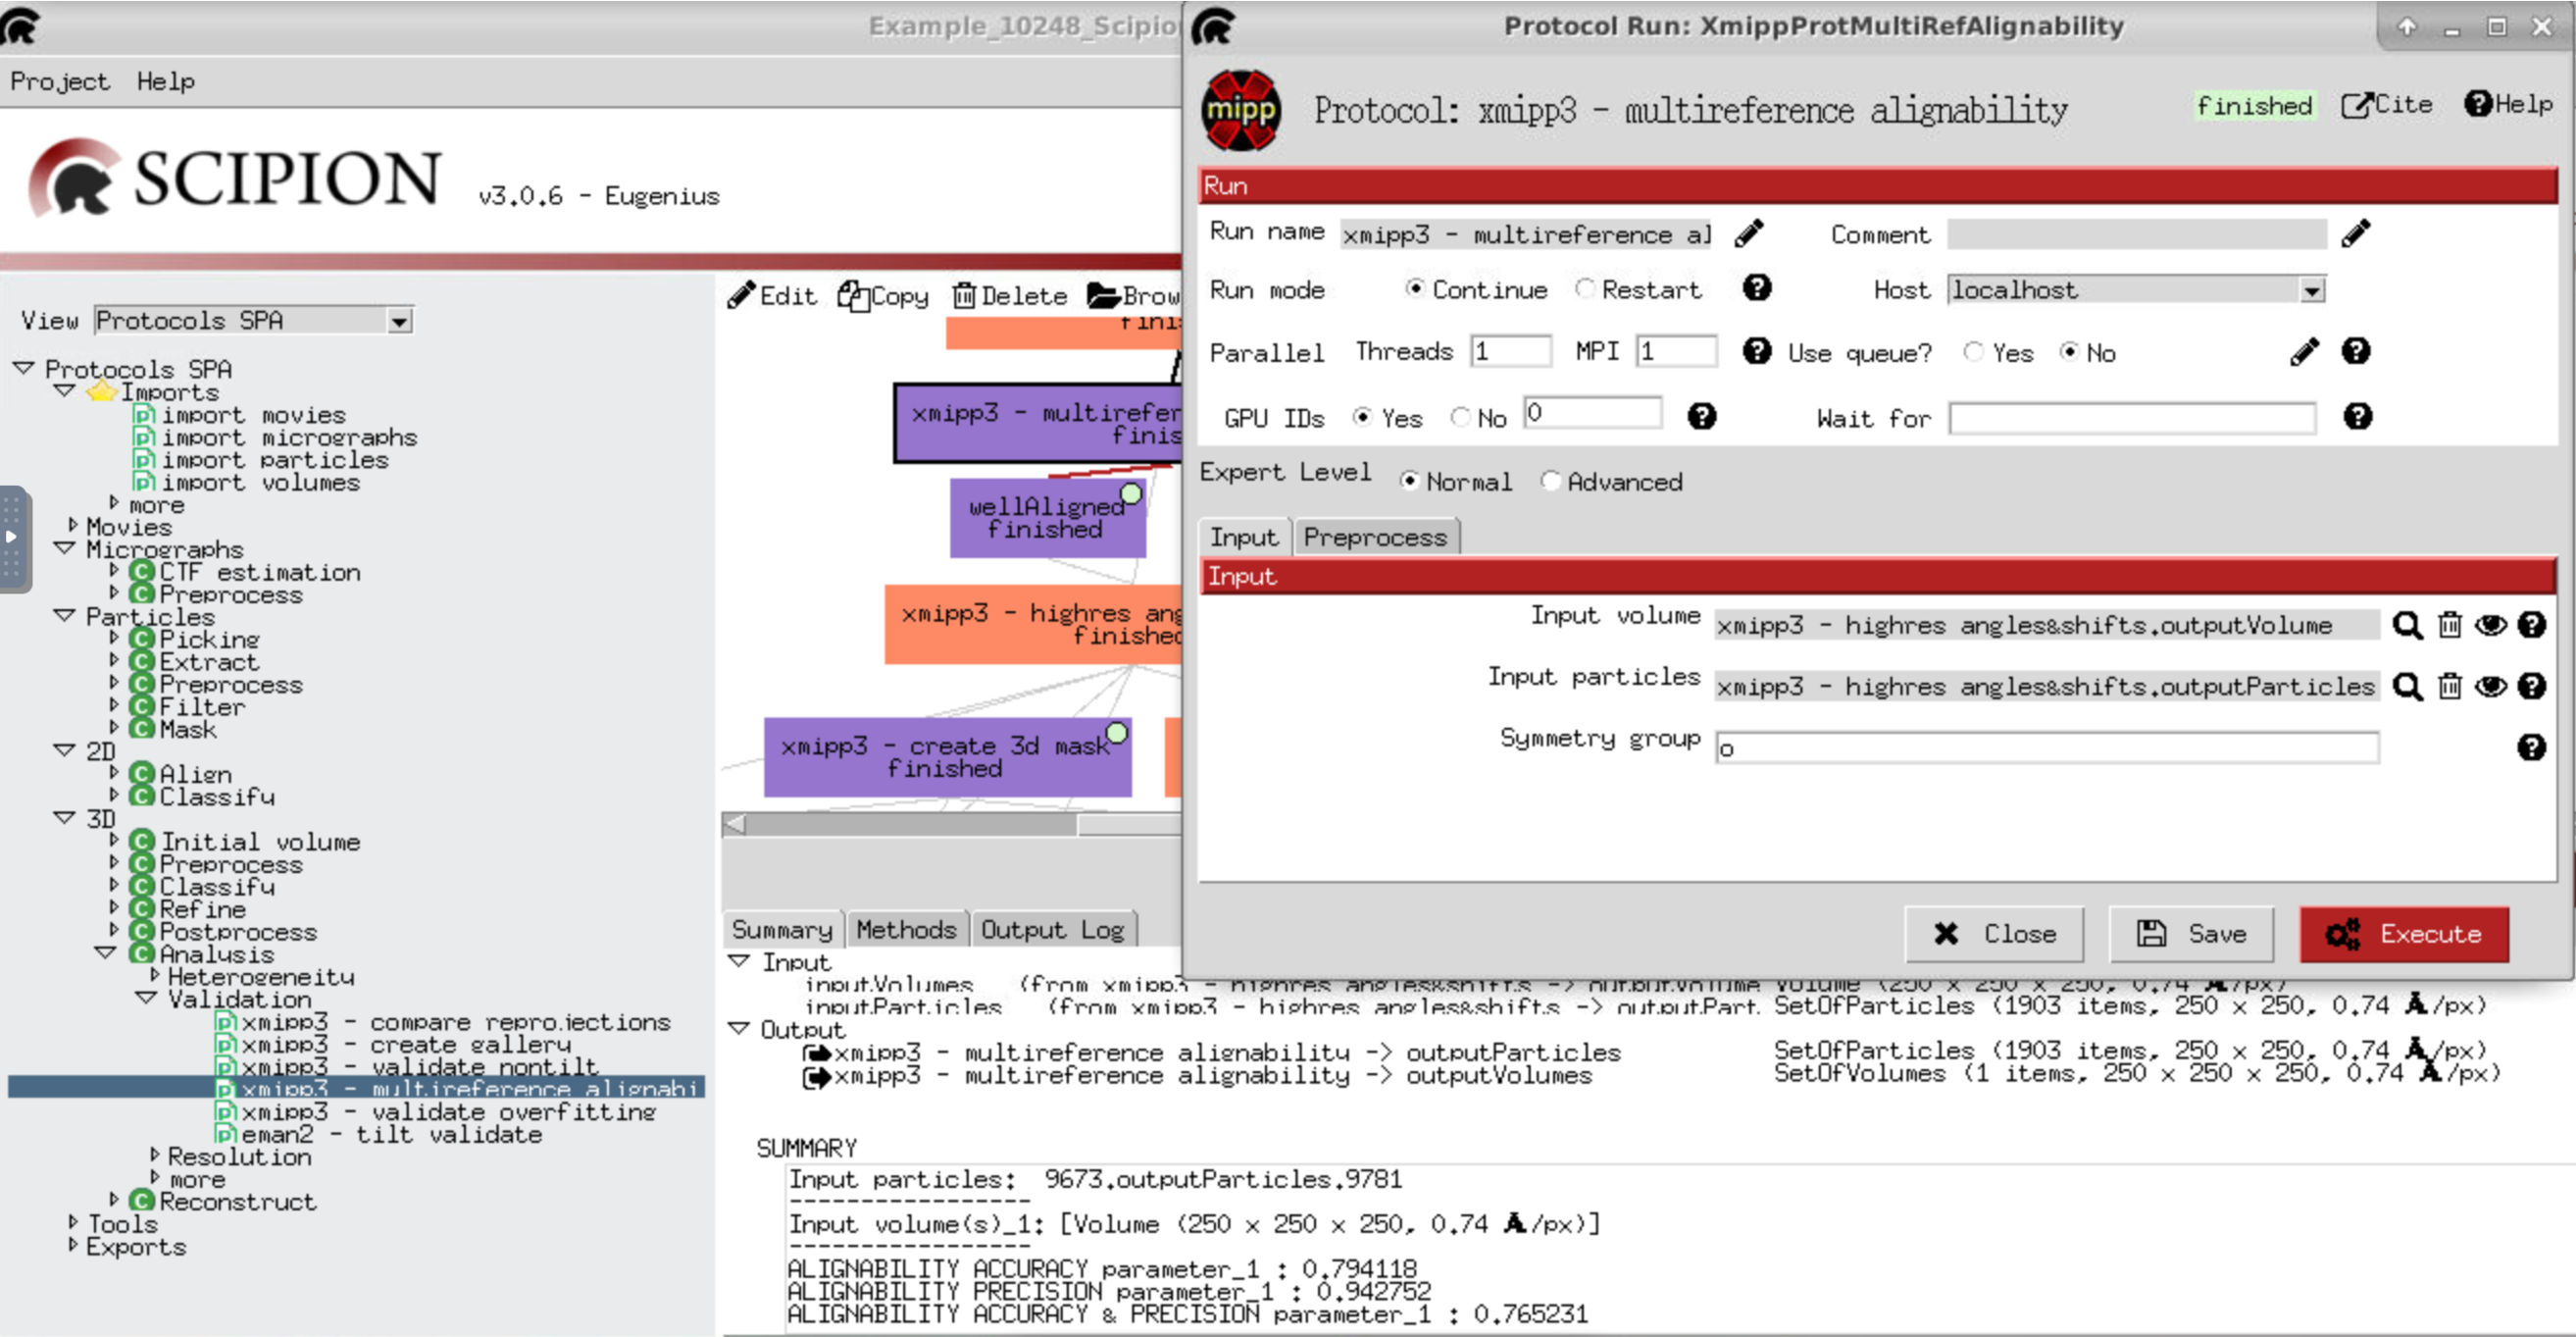
\includegraphics[width=0.95\textwidth]
  {{images/10a_xmipp3_multiRefAlign.pdf}}
  \caption{Completing the form of protocol \scommand{xmipp3-multireference alignability}.}
  \label{fig:multireference_alignability}
  \end{figure}

The output values of particle alignment, precision and accuracy, generated by \scommand{xmipp3-multireference alignability} (press \scommand{Analyze Results}) allow us to discard particles with worse alignment. In this case, 446 particles (23.4\% of the total input) are rejected. A new subset of 1,457 particles will be created included in the box \ttt{wellAligned}. In order to improve the refined map resolution, the remaining 1,457 particles will be used to perform the local refinement iteration with $Xmipp$ \ttt{highres} algorithm. The protocol params will remain unchanged compared with the first implementation.

\begin{figure}[H]
  \centering
  \captionsetup{width=.8\linewidth} 
  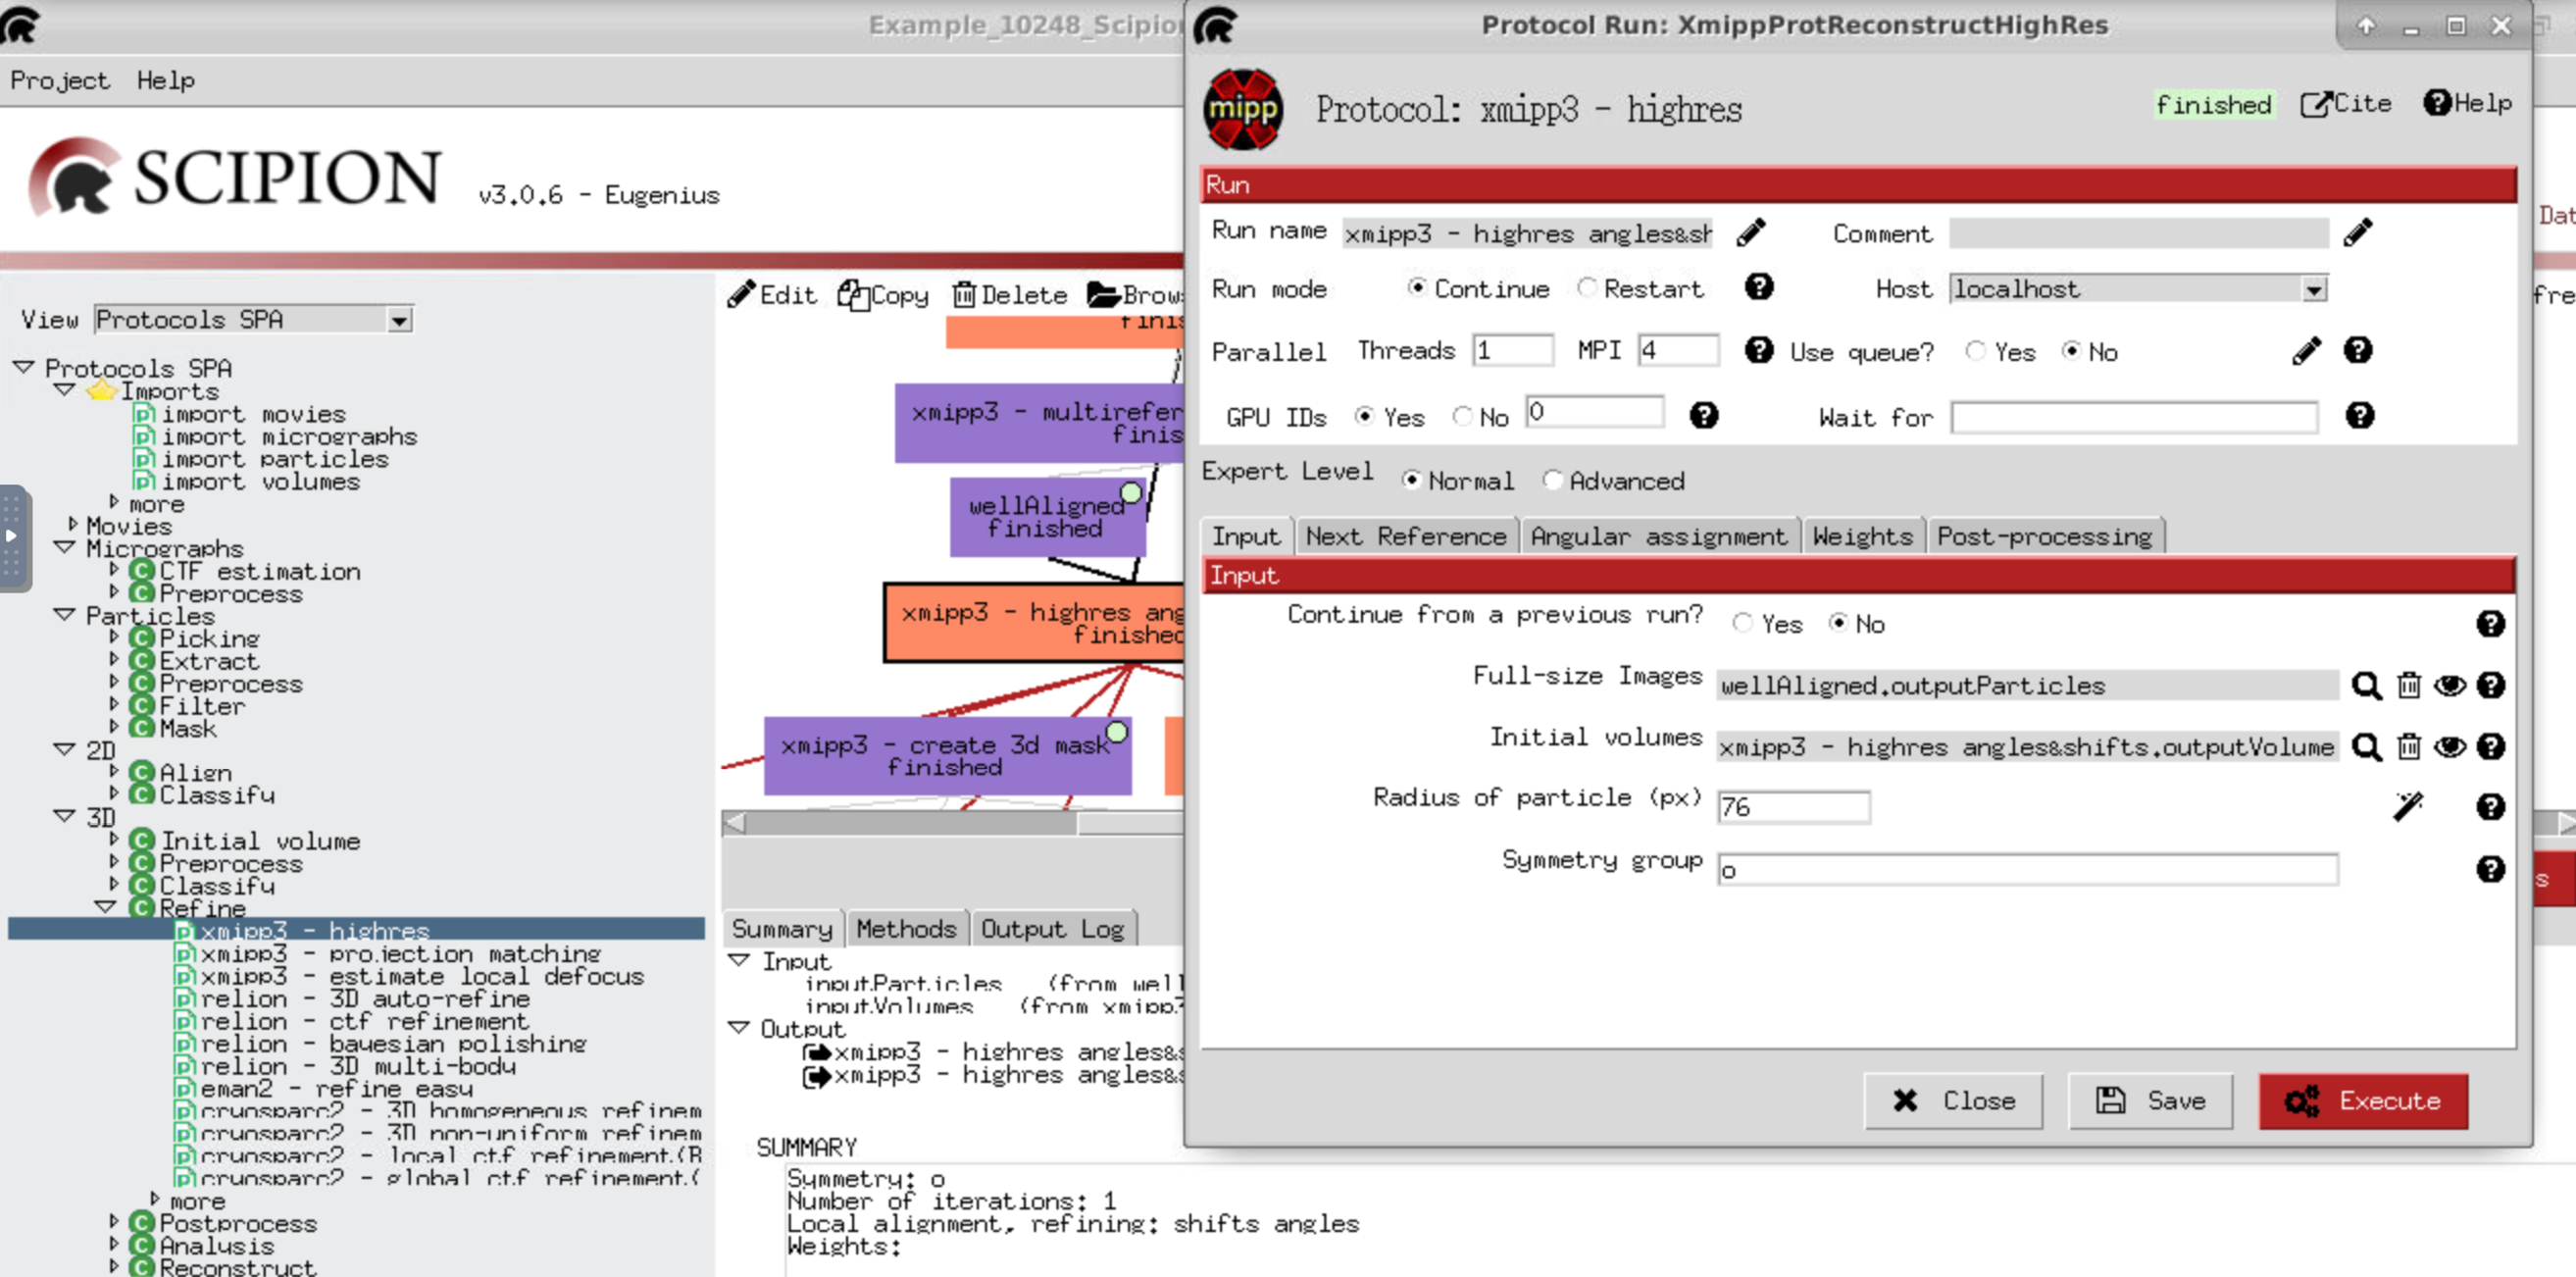
\includegraphics[width=0.95\textwidth]
  {{images/10b_xmipp3_highres2.pdf}}
  \caption{$Xmipp$ \ttt{highres}.}
  \label{fig:highres_fullsize6}
  \end{figure}

The sampling of the output map is the same than in the previous implementation, despite the selection of best aligned particles. We have thus achieved convergence and we can compute the global or local resolution for sharpening the map. Map sharpening contributes to increase signal at medium/high resolution, we recommend to perform this map preprocessing step before tracing the atomic model of cryo-EM 3D maps. To accomplish this task a couple of automatic alternatives are available in Scipion: a) local sharpening method independent of initial model, based on local resolution estimation \scommand{xmipp3 - localdeblur sharpening} (Ramírez-Aportela et al., 2018), b) deep learning-based sharpening approach \scommand{xmipp3 - deepEMhancer} (Sanchez-Garcia et al., 2020). Although both sharpening methods display good results, these are not identical but complementary since LocalDeblur maximizes specially details like the secondary structure, whereas DeepEMhancer maximizes connectivity, favoring the fair tracing of the molecule skeleton.\\

\subsection*{Map sharpening: a) Local sharpening method independent of initial model, based on local resolution estimation}

At this point, we may define a mask, and this mask will help directional resolution and local resolution algorithms to concentrate on which area they should analyze. Basically it is used to see the distribution of the noise and know where is the noise to get rid of it. For this we will use the protocol \scommand{xmipp3-create 3D mask}, the mask can be created with a given geometrical shape (Sphere, Box, Cylinder...) or it can be obtained from operating on a 3D volume or a previous mask. In this case it comes from the previous 3D volume as you can see in the next figure \ffigure{fig:create_3Dmask}.

\begin{figure}[H]
  \centering
  \captionsetup{width=.8\linewidth} 
  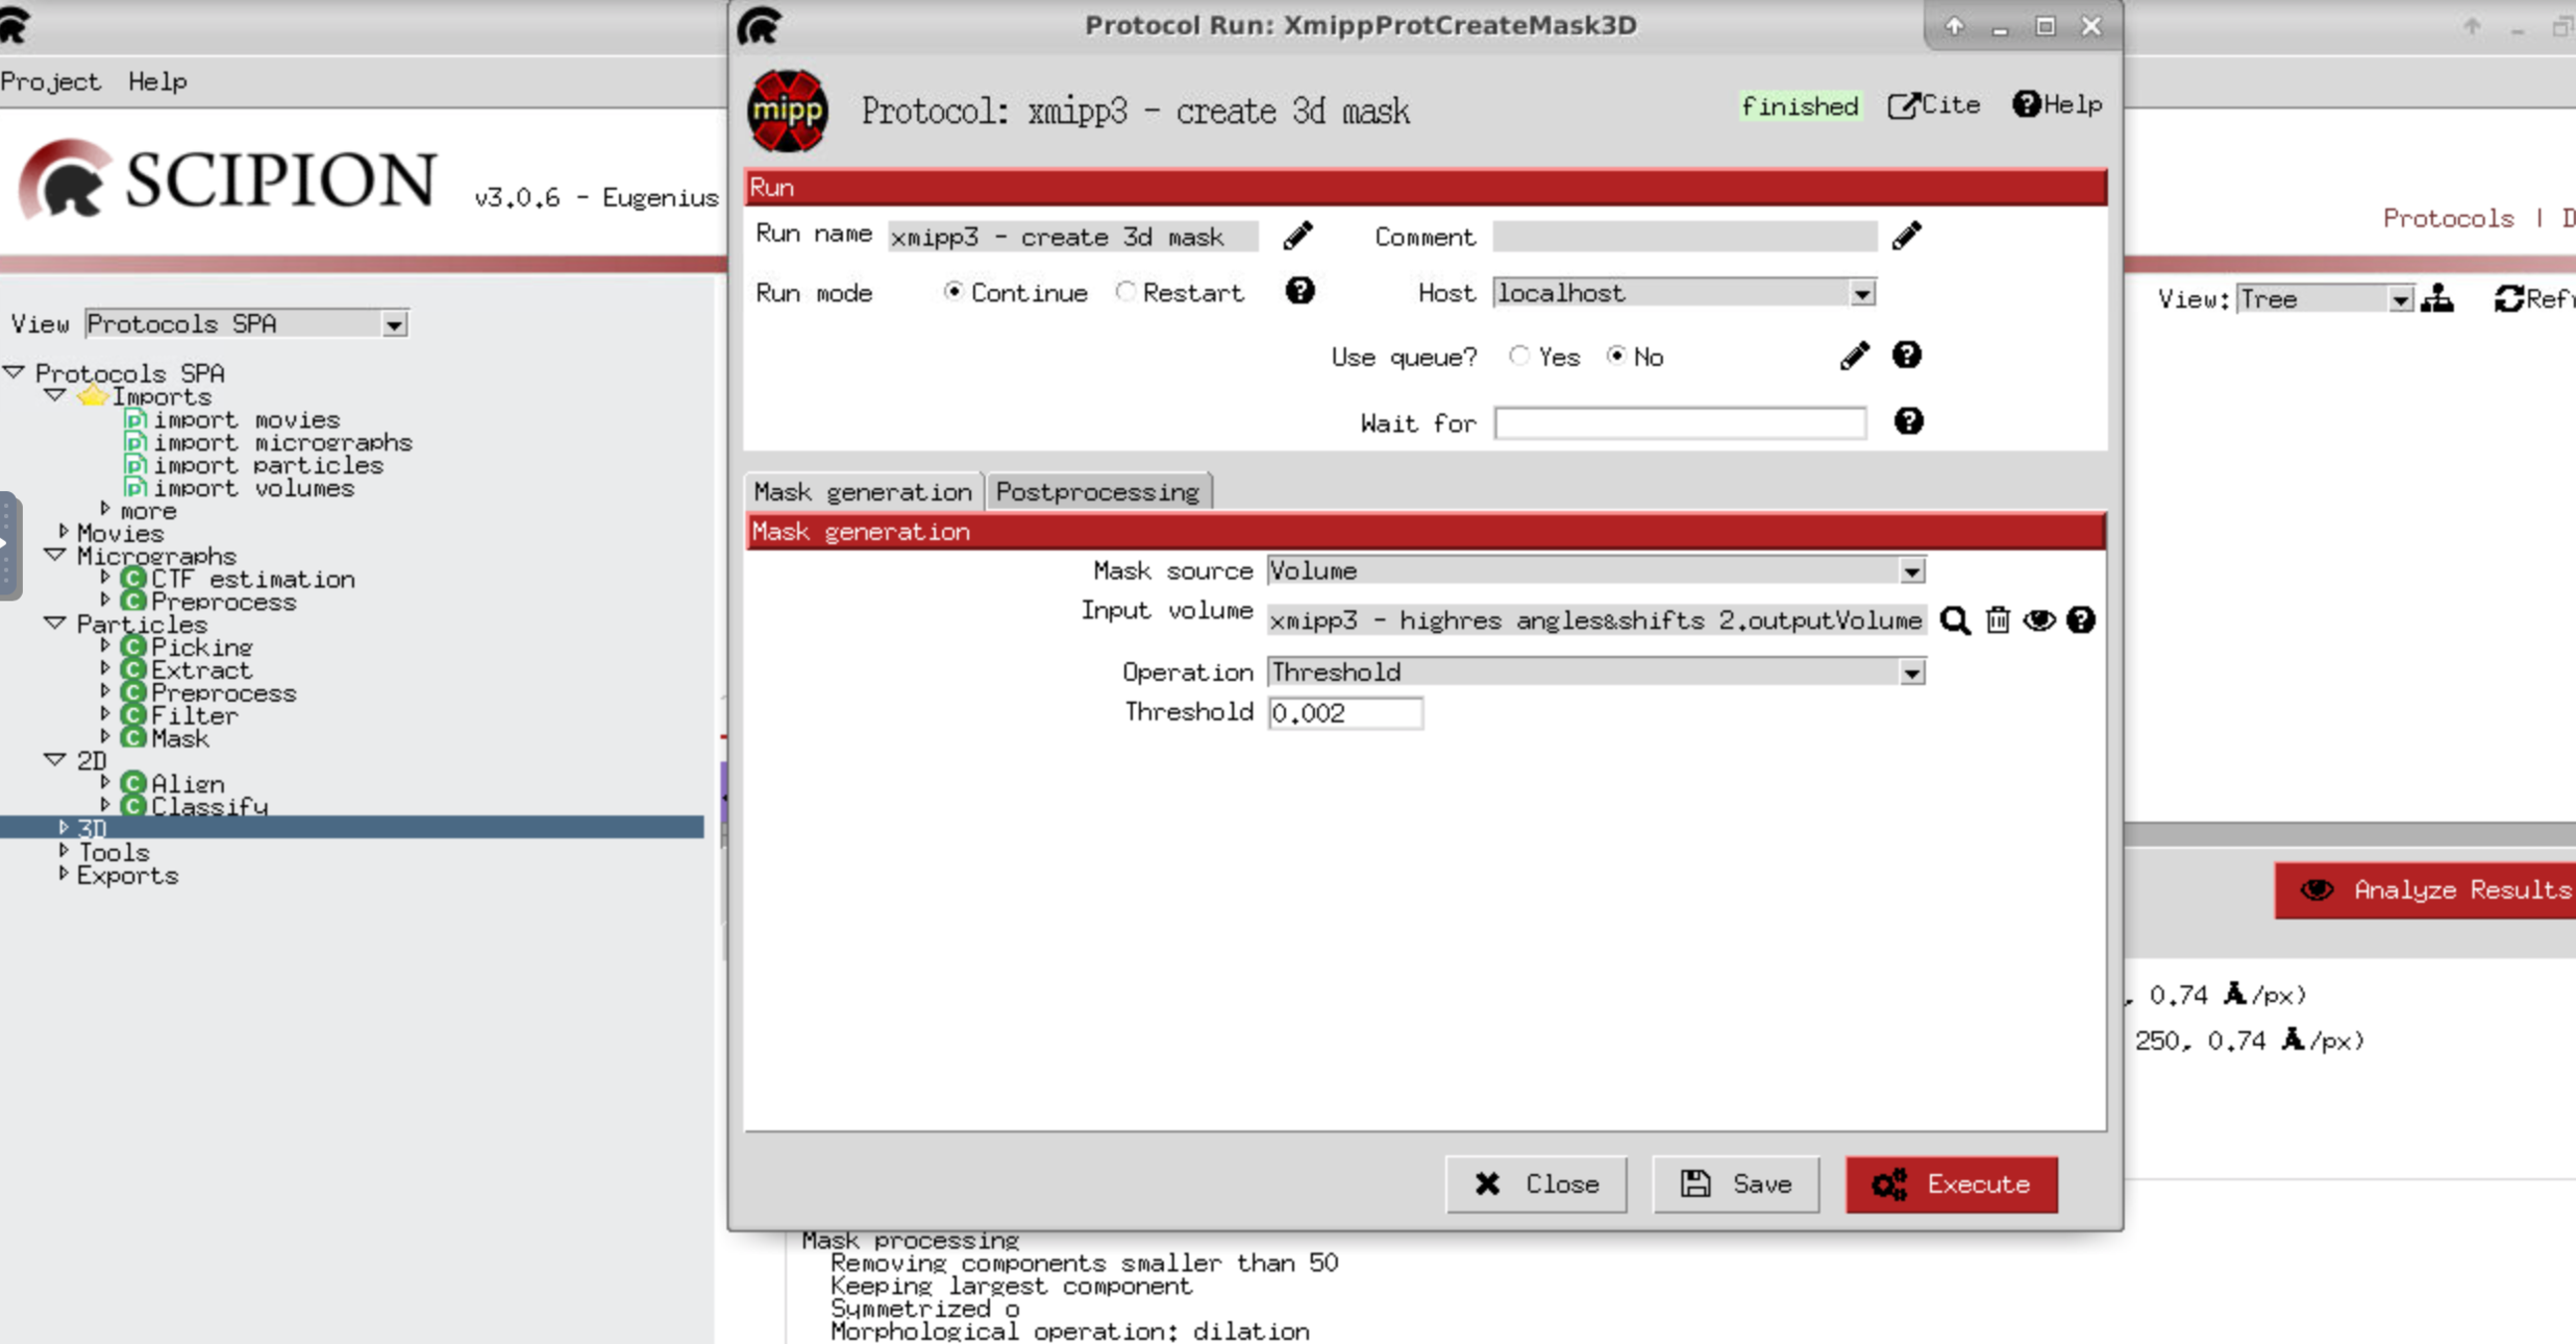
\includegraphics[width=0.95\textwidth]
  {{images/10c_xmipp3_create3Dmask.pdf}}
  \caption{$Xmipp$ \ttt{create 3Dmask}.}
  \label{fig:create_3Dmask}
  \end{figure}
 
Once the map mask is created, the protocol \scommand{xmipp3-local deepRes} (\ffigure{fig:local_deepRes1}) can be completed to get the estimation of local resolution. We have to include the input volume, as well as the binary mask and finally, based on the map resolution (3.2 \AA\ ), select the default resolution range between 2.5\AA\ and 13\AA\ . Given a map the protocol will assign local resolutions to each voxel of the map.  

\begin{figure}[H]
  \centering
  \captionsetup{width=.8\linewidth} 
  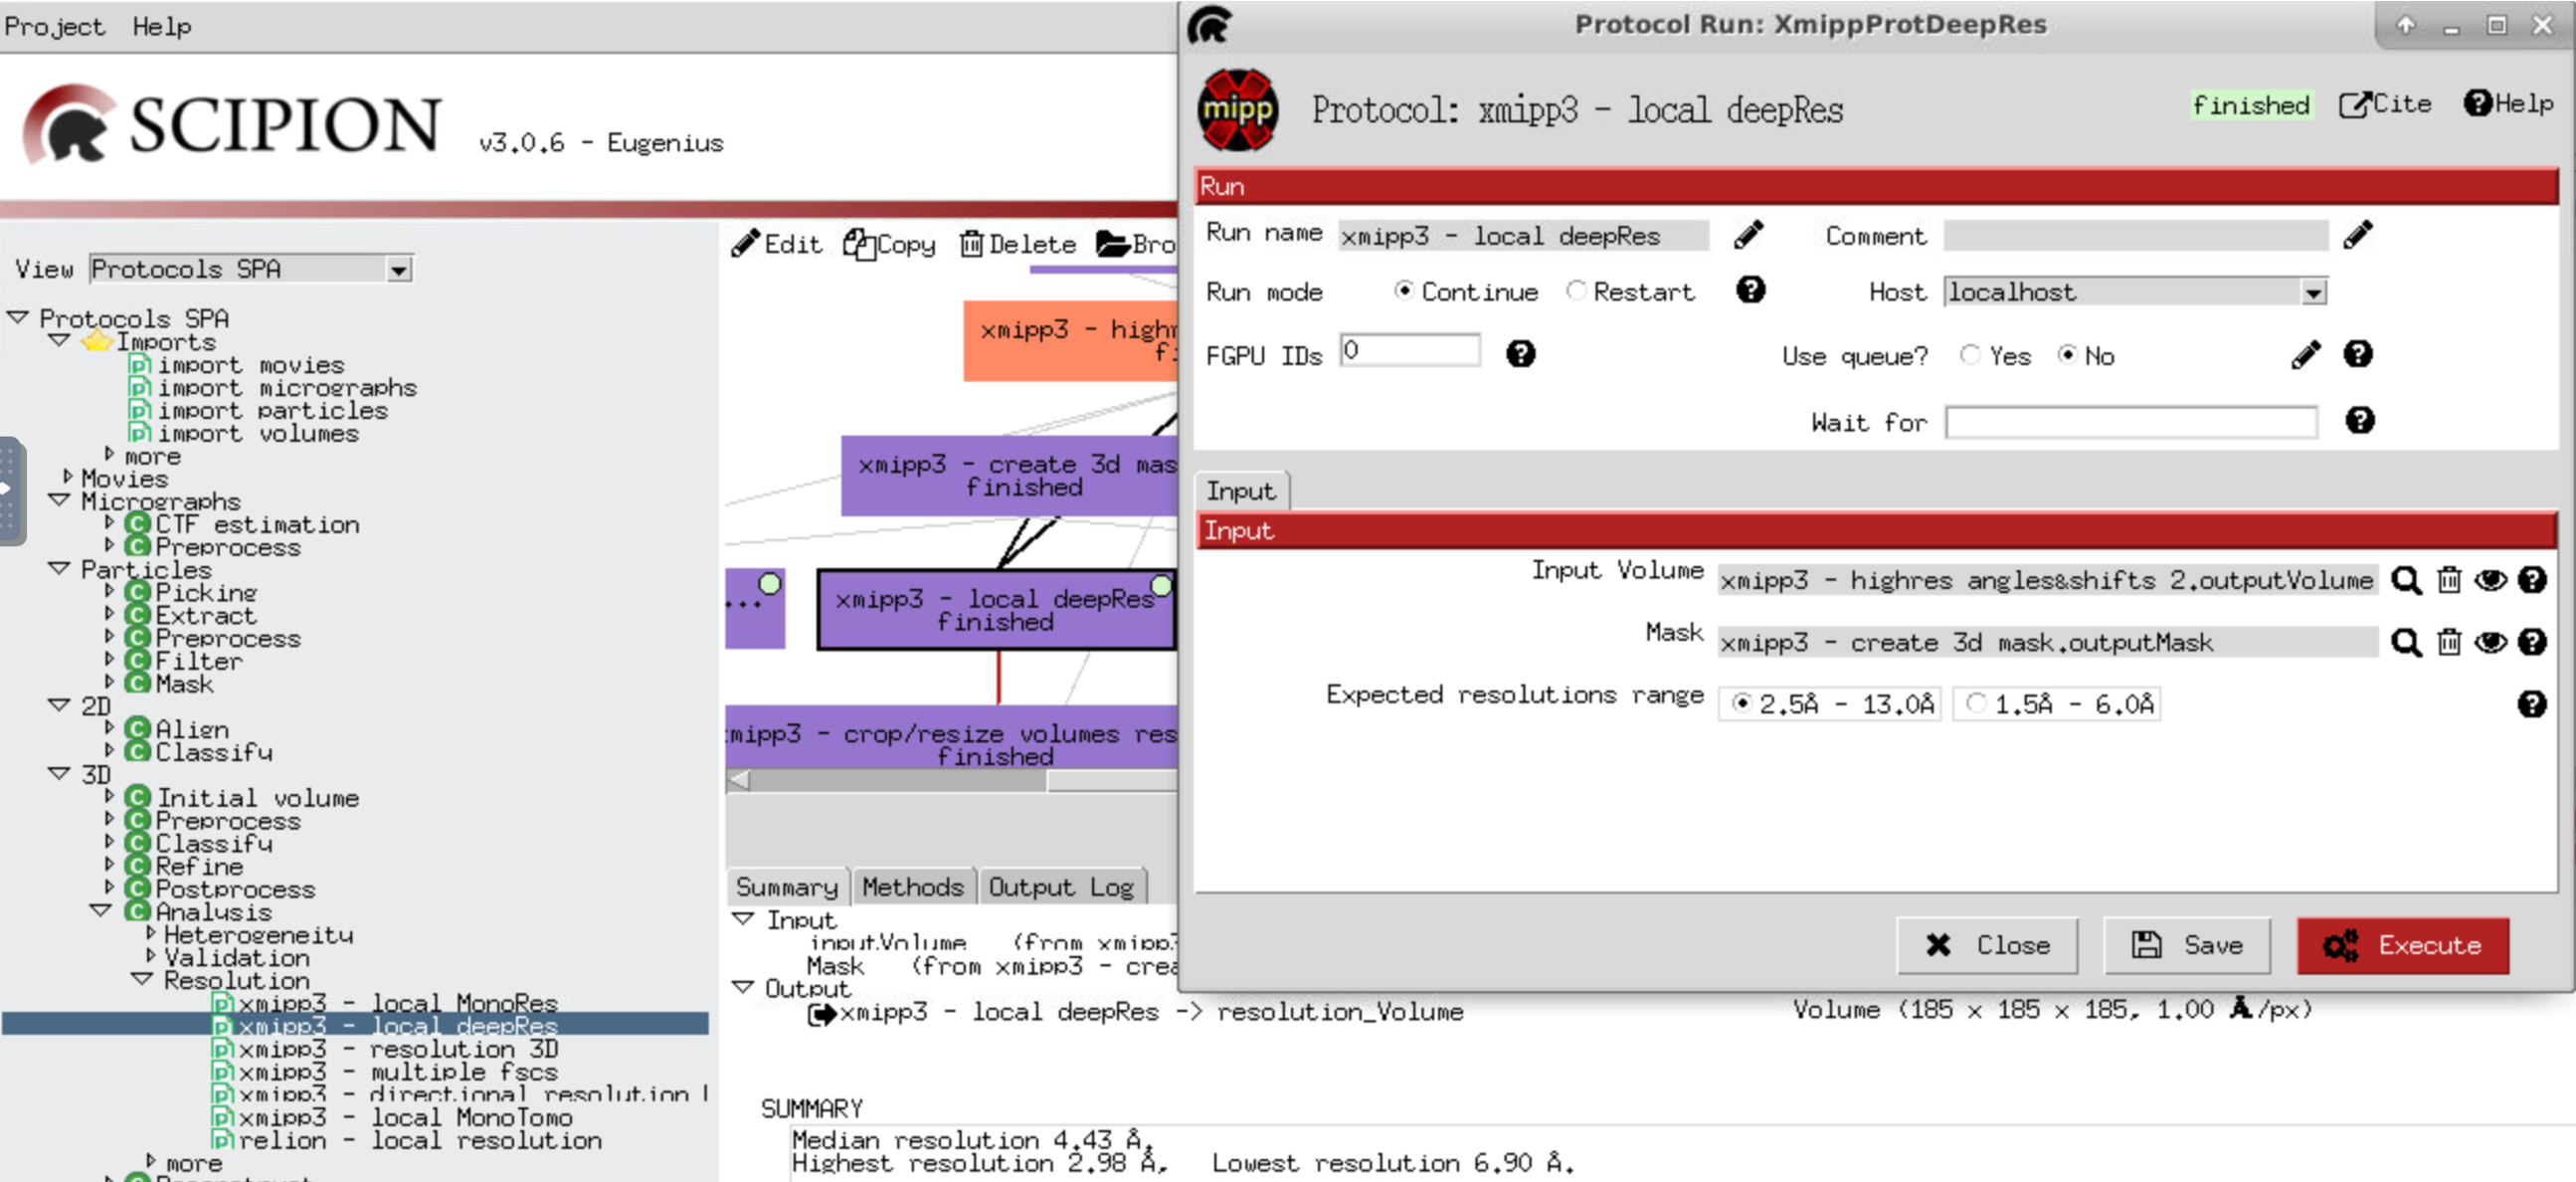
\includegraphics[width=0.95\textwidth]
  {{images/10f_xmipp3_localdeepRes.pdf}}
  \caption{$Xmipp$ \ttt{local deepRes} .}
  \label{fig:local_deepRes1}
  \end{figure}
 
 Press \scommand{Analyze Results}  to see the menu of results, among other views, it shows the histogram of local resolutions and the resolution map in ChimeraX. The histogram of resolutions, which displays the number of map voxels showing a certain resolution, allows us to conclude that the majority of voxels evidence a resolution between 4.2\AA\ .The resolution map shown by ChimeraX details the resolution of each voxel by colors.\\
 
 Resolution is not only local but also directional, in different directions you can have different resolution. To compute this difference, we used \scommand{xmipp3-directional resolution MonoDir} protocol (\ffigure{fig:dir_Res}).
 
 \begin{figure}[H]
  \centering
  \captionsetup{width=.8\linewidth} 
  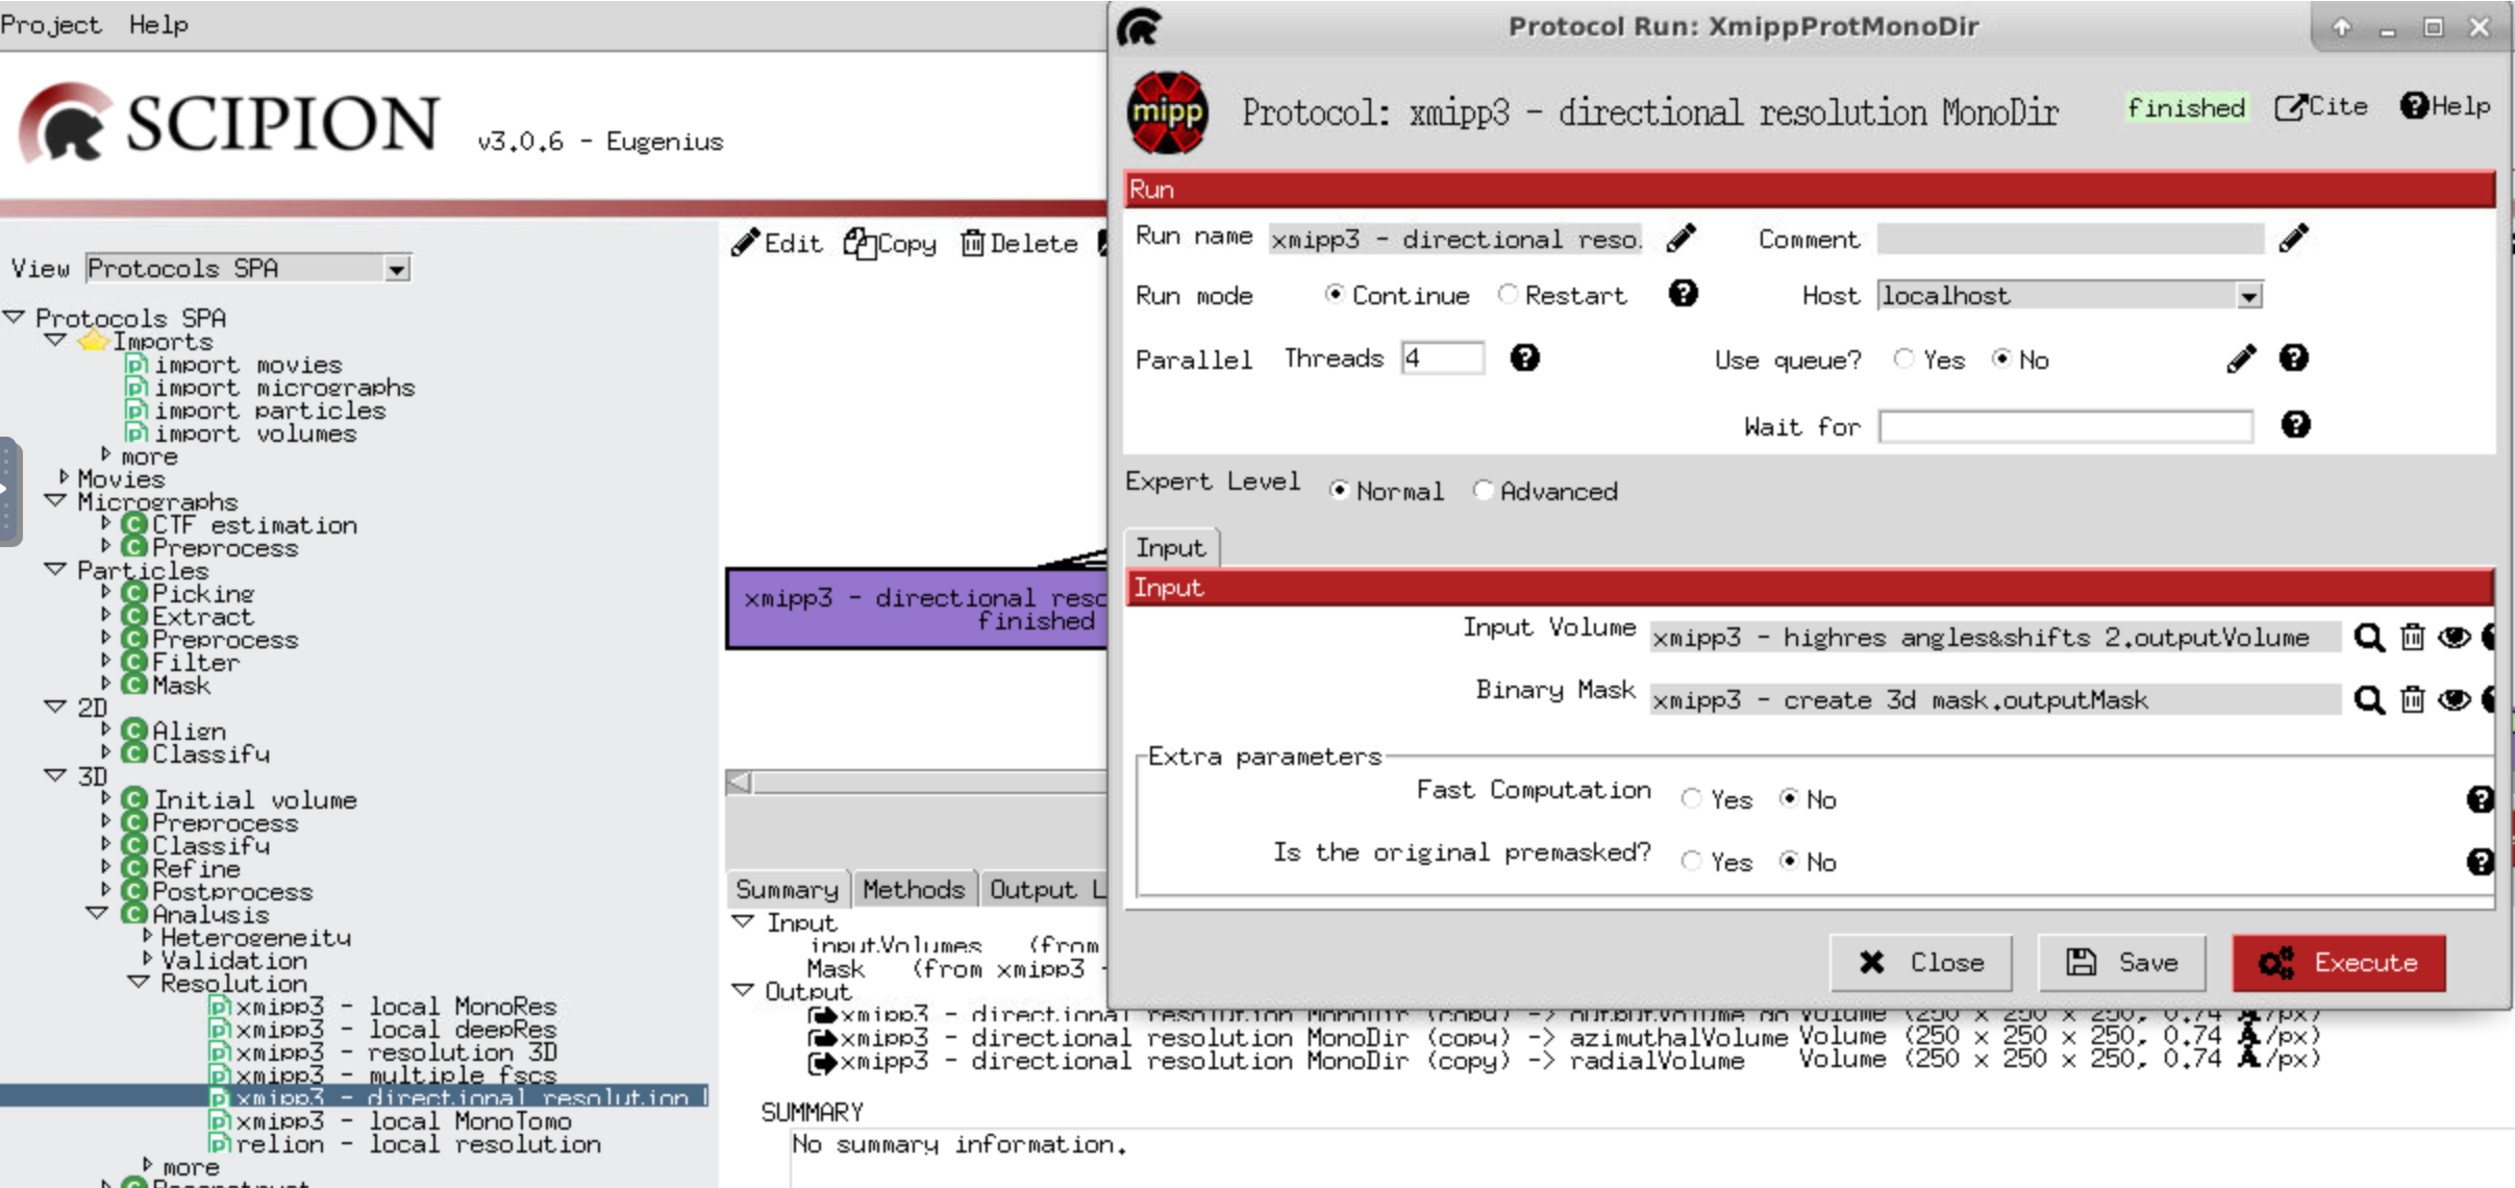
\includegraphics[width=0.95\textwidth]
  {{images/10e_xmipp3_dir_resolution.pdf}}
  \caption{$Xmipp$ \ttt{directional resolution MonoDir}.}
  \label{fig:dir_Res}
  \end{figure} 
 
 The interesting views of \scommand{Analyze Results} are, the \ttt{Half Interquartile Range} between different resolutions. In this case we can appreciate that the region of the structure looks very consistent and all the inconsistency comes from the surrounding. Another interesting plot is the \ttt{Directions histogram}, basically how many voxels have their maximum resolution along that direction. In this case it looks uniform and this can be confirmed by looking to the \ttt{radial averages} (radial averages of the resolutions in different directions).\\
 
Back to the sharpening of the map, local resolution values of the input map allow to compute the sharpened map by \scommand{xmipp3-localdeblur sharpenning} protocol, which implements an iterative steep descending method that not requires initial model. To accomplish this step, first we have to resize our resolution volume since \scommand{xmipp3-local deepRes} computed a resolution volume with different dimensions and sampling frequency than our actual volume. To do so, we use \scommand{xmipp-crop/resize} protocol on the volume resolution to obtain 250x250x250 dimensions and 0.74\AA\ /px sampling rate (\ffigure{fig:xmipp_crs1}).

 \begin{figure}[H]
  \centering
  \captionsetup{width=.8\linewidth} 
  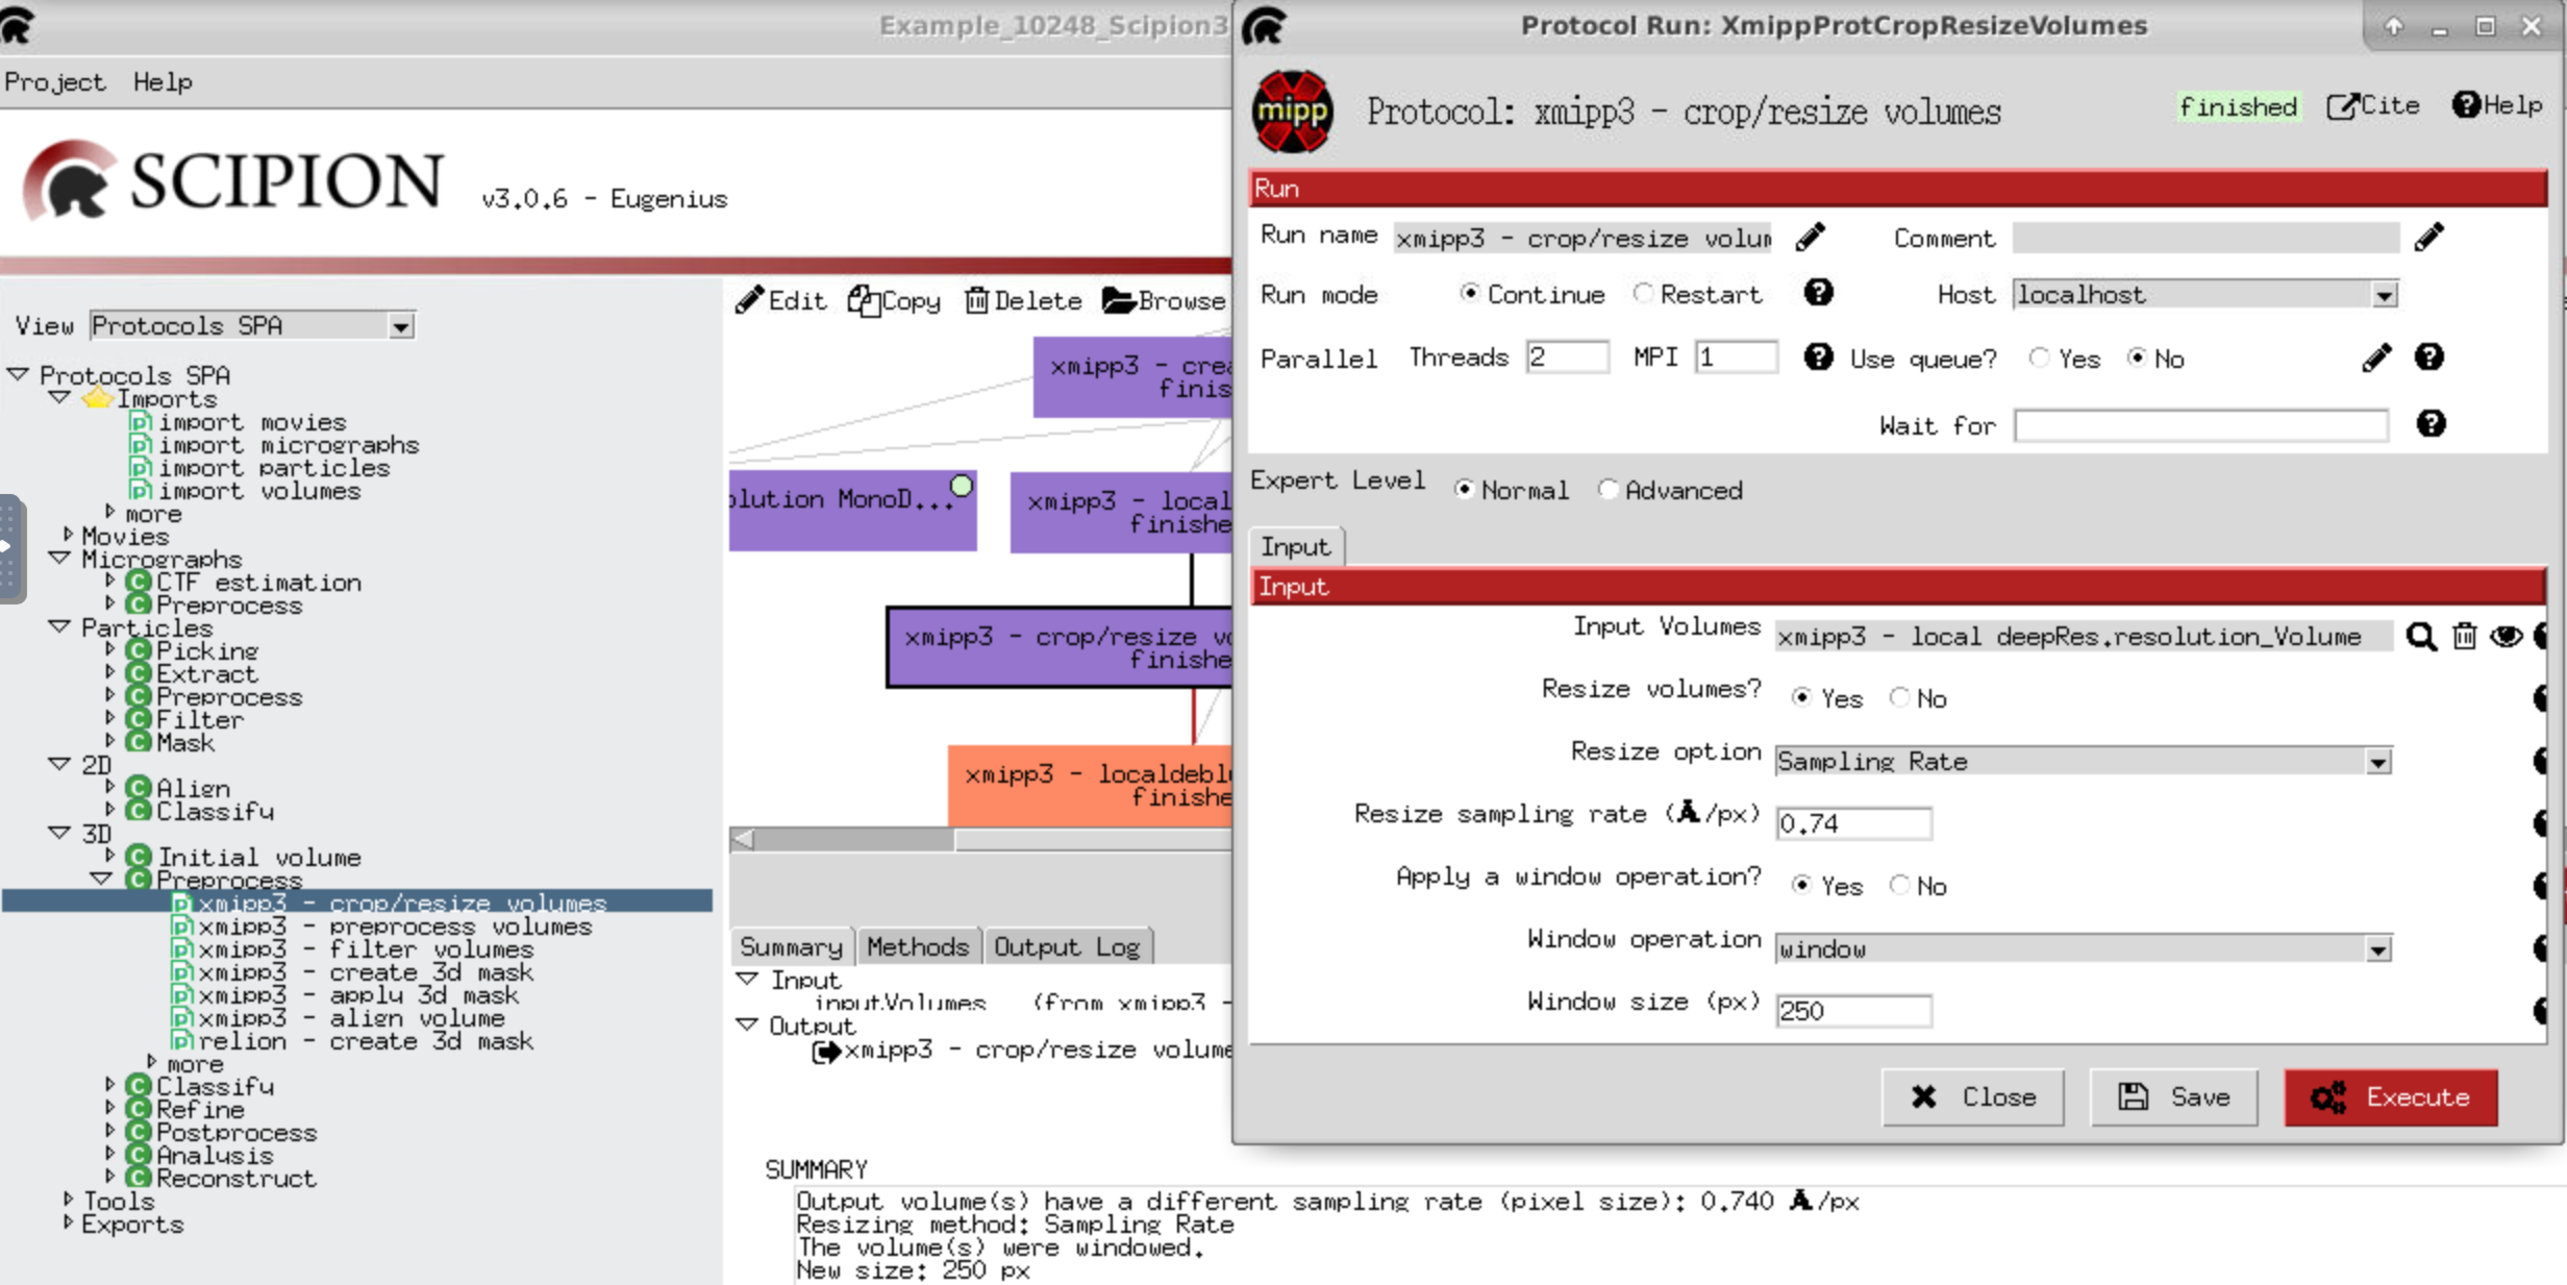
\includegraphics[width=0.95\textwidth]
  {{images/10h_xmipp3_cropresize1.pdf}}
  \caption{$Xmipp$ \ttt{crop/resize}.}
  \label{fig:xmipp_crs1}
  \end{figure} 
  
LocalDeblur takes advantage of the map local resolution to increase the signal, so as input of \scommand{xmipp3-localdeblur sharpenning} protocol we should include the starting map and the map of resolution values, maintaining the default values for the rest of parameters (\ffigure{fig:xmipp_localdeblur1}). 

 \begin{figure}[H]
  \centering
  \captionsetup{width=.8\linewidth} 
  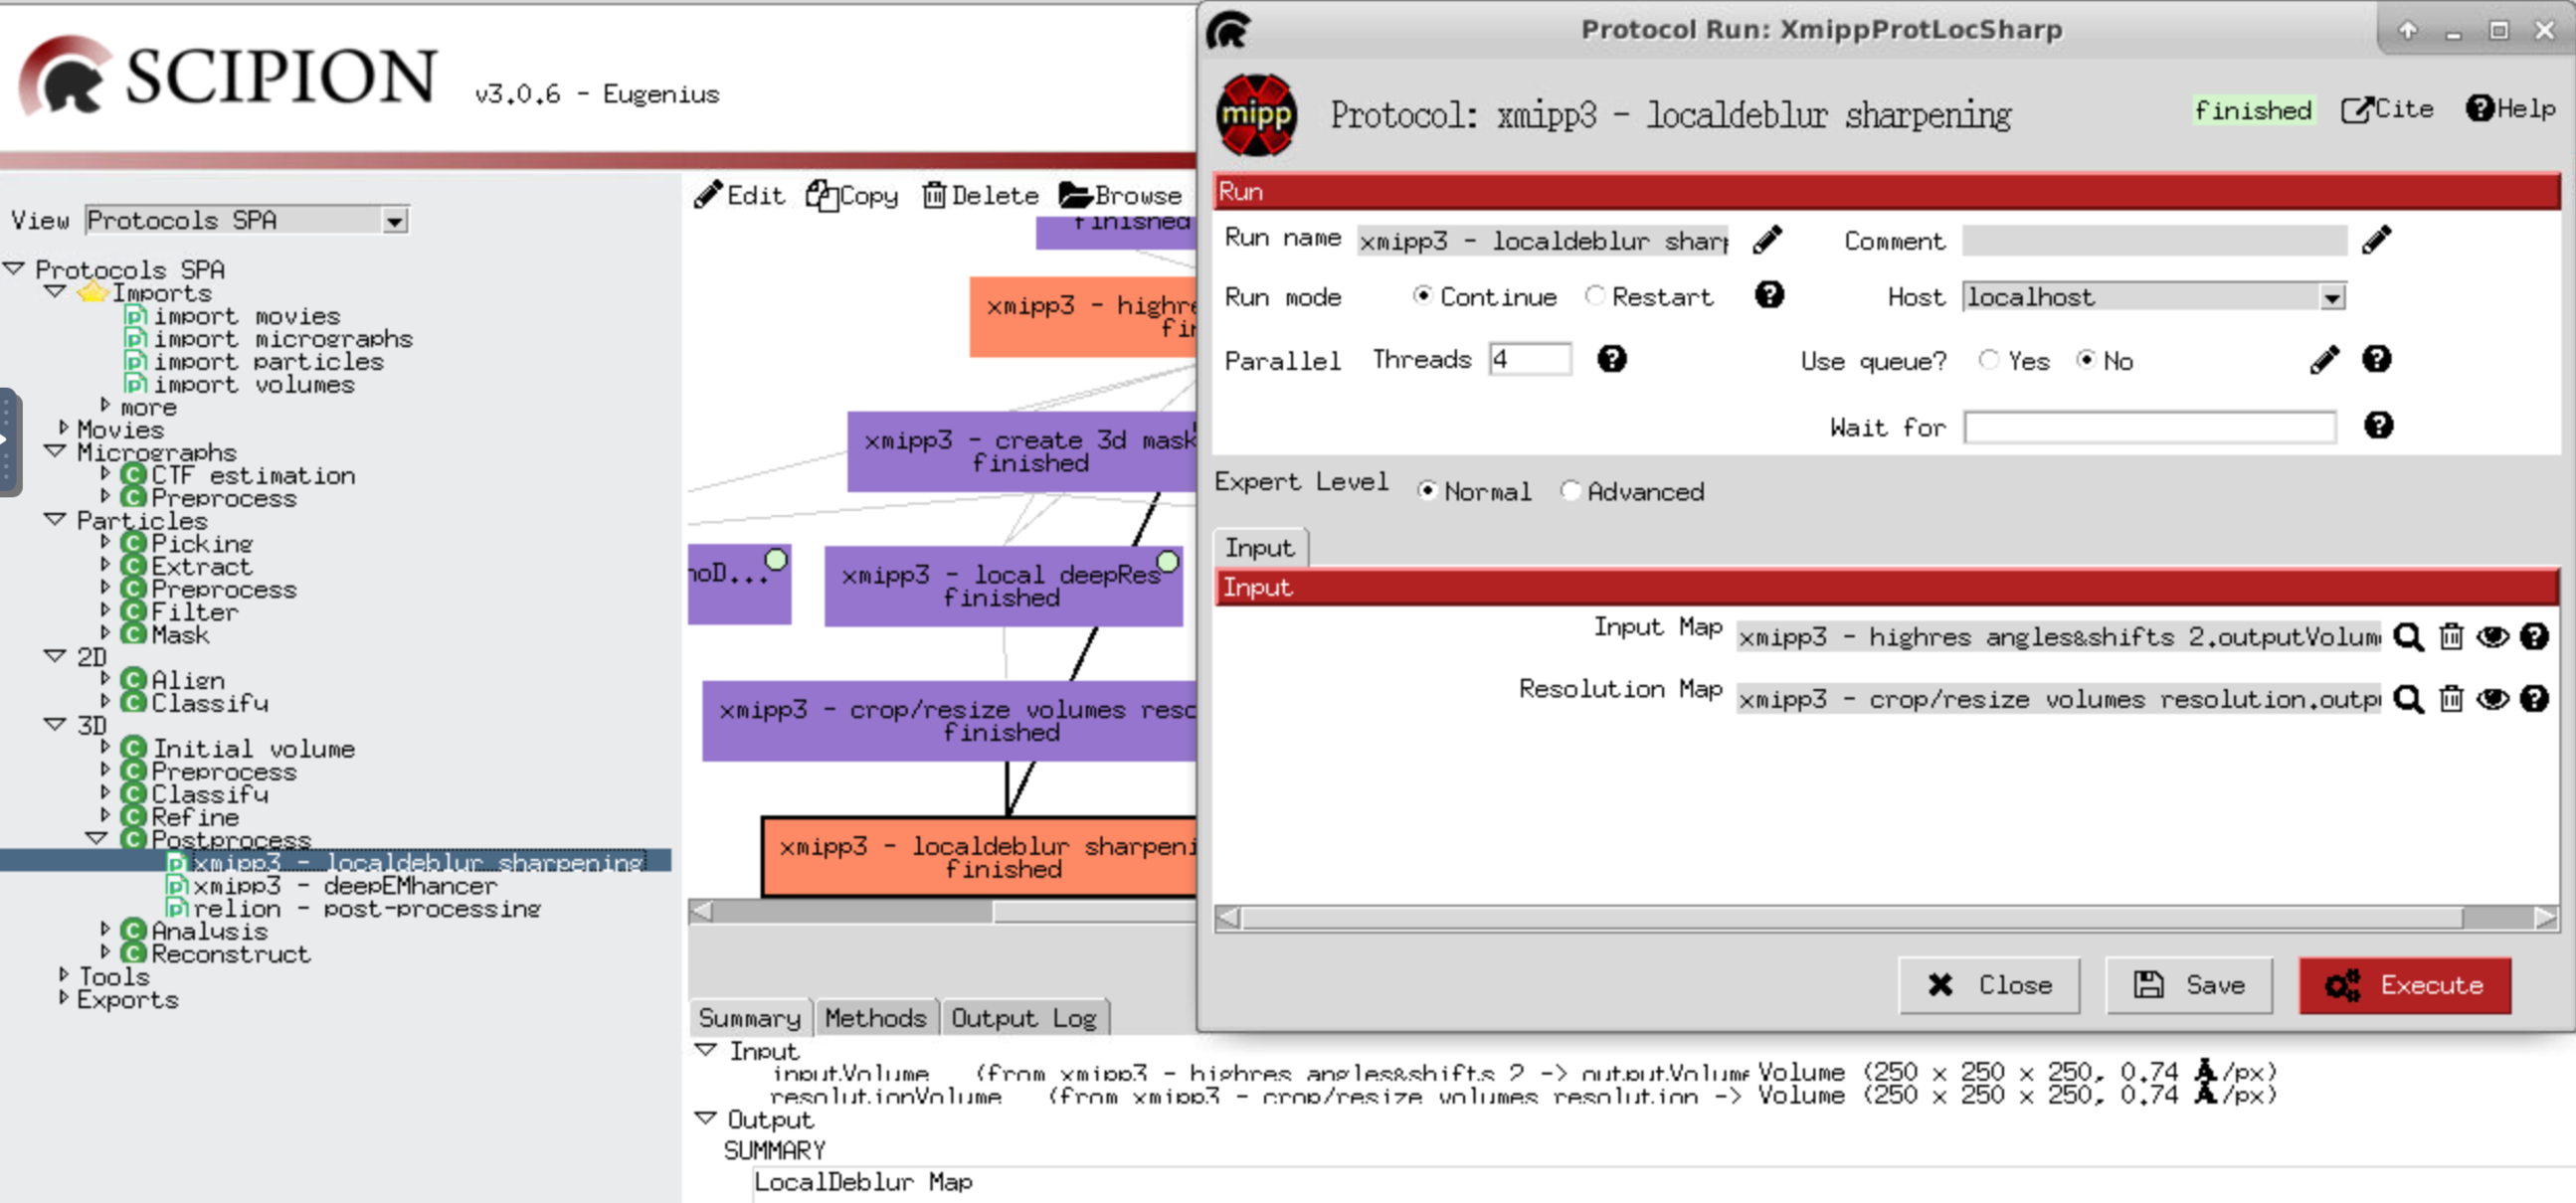
\includegraphics[width=0.95\textwidth]
  {{images/10j_xmipp3_localdeblur1.pdf}}
  \caption{$Xmipp$ \ttt{localdeblur sharpenning}.}
  \label{fig:xmipp_localdeblur1}
  \end{figure} 
  
  After three iterations, the sharpening algorithm reached the convergence criterion, i.e. a difference between two successive iterations lower than 1\% and stopped. The three maps obtained in the respective iterations can be observed with double-clicking the black output arrow shown in the summary. Additionally, by clicking \scommand{Analyze Results} the sharpened map obtained after the third iteration, i.e. the last map, can be also visualized and compared with the initial one in ChimeraX.
  
  \subsection*{Map sharpening: b) deep learning-based approach}
  
DeepEMhancer is an alternative automatic sharpening method based on deep learning (Sanchez-Garcia et al., 2020), implemented in Scipion in the protocol \scommand{xmipp3-deepEMhancer}. Given a map the protocol performs automatic deep post-processing to enhance visualization. We have to include the map, the type of normalization desired and the deep learning mode to use, in this particular case tight target (\ffigure{fig:xmipp_deepEM}).

 \begin{figure}[H]
  \centering
  \captionsetup{width=.8\linewidth} 
  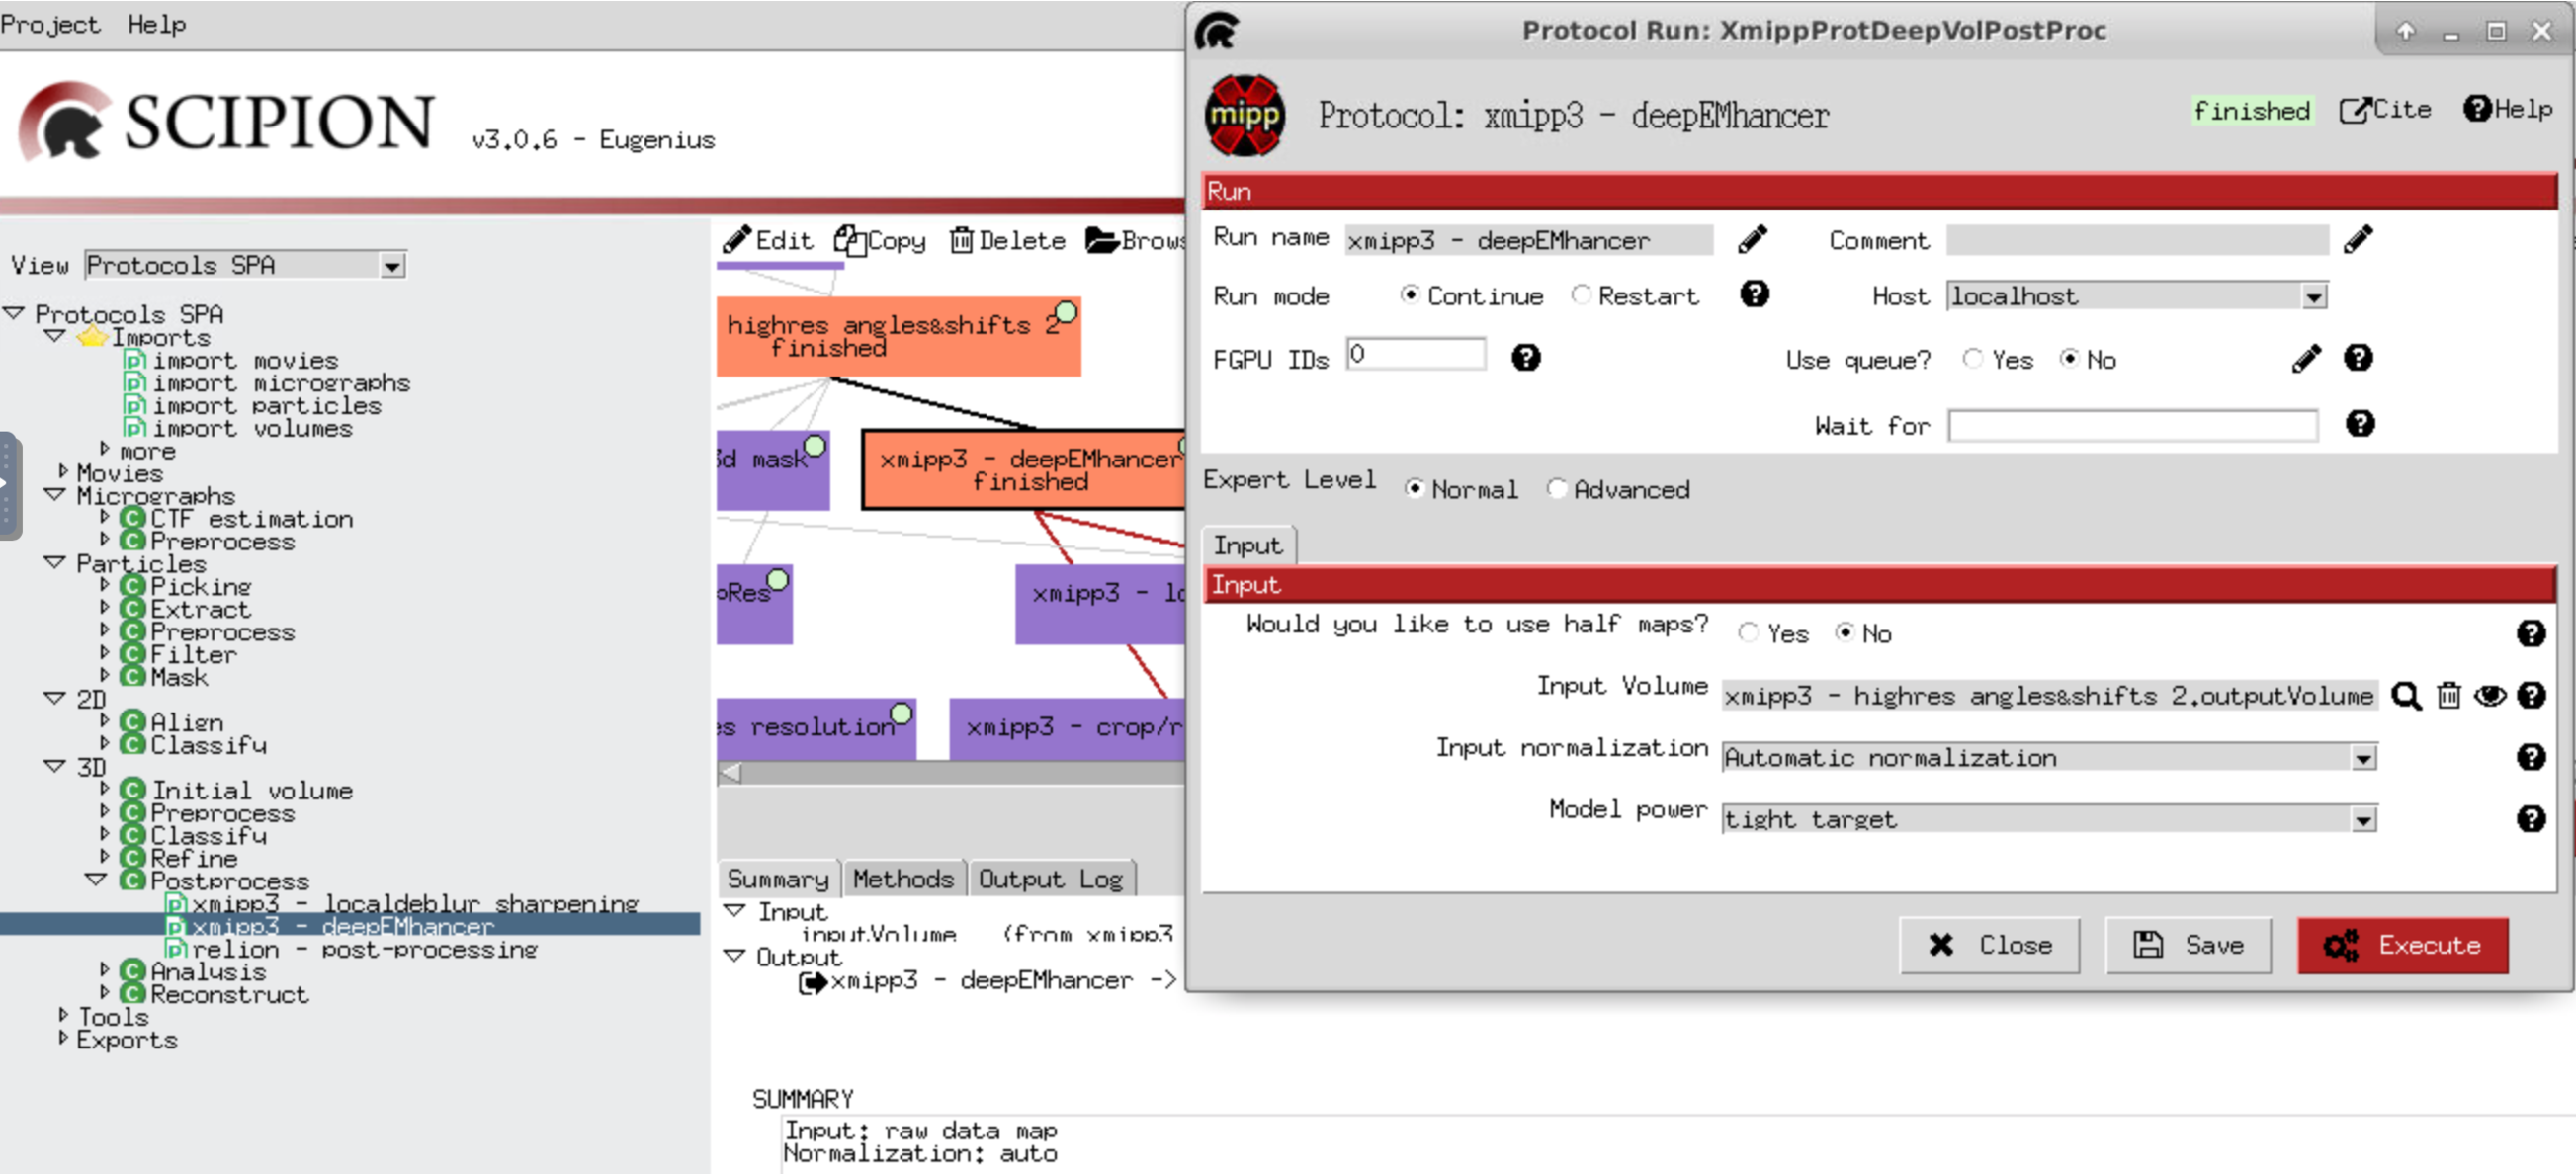
\includegraphics[width=0.95\textwidth]
  {{images/10d_xmipp3_deepEMenhancer.pdf}}
  \caption{$Xmipp$ \ttt{deep EMhancer}.}
  \label{fig:xmipp_deepEM}
  \end{figure} 

After executing the protocol with \scommand{Analyze Results} , we can check the results. ChimeraX viewer will open and show the sharpened map compared with the initial one.\\

 For further refinement, we can compute the local estimation as it was done before with \scommand{xmipp3-local deepRes} (\ffigure{fig:xmipp_localdeepRes2}), then the resolution volume output is resized again with \scommand{xmipp-crop/resize} protocol  (\ffigure{fig:xmipp_croprs2}) and we can restore the map running \scommand{xmipp3-localdeblur sharpening} protocol (\ffigure{fig:xmipp_localdeblur2}).  
 
  \begin{figure}[H]
  \centering
  \captionsetup{width=.8\linewidth} 
  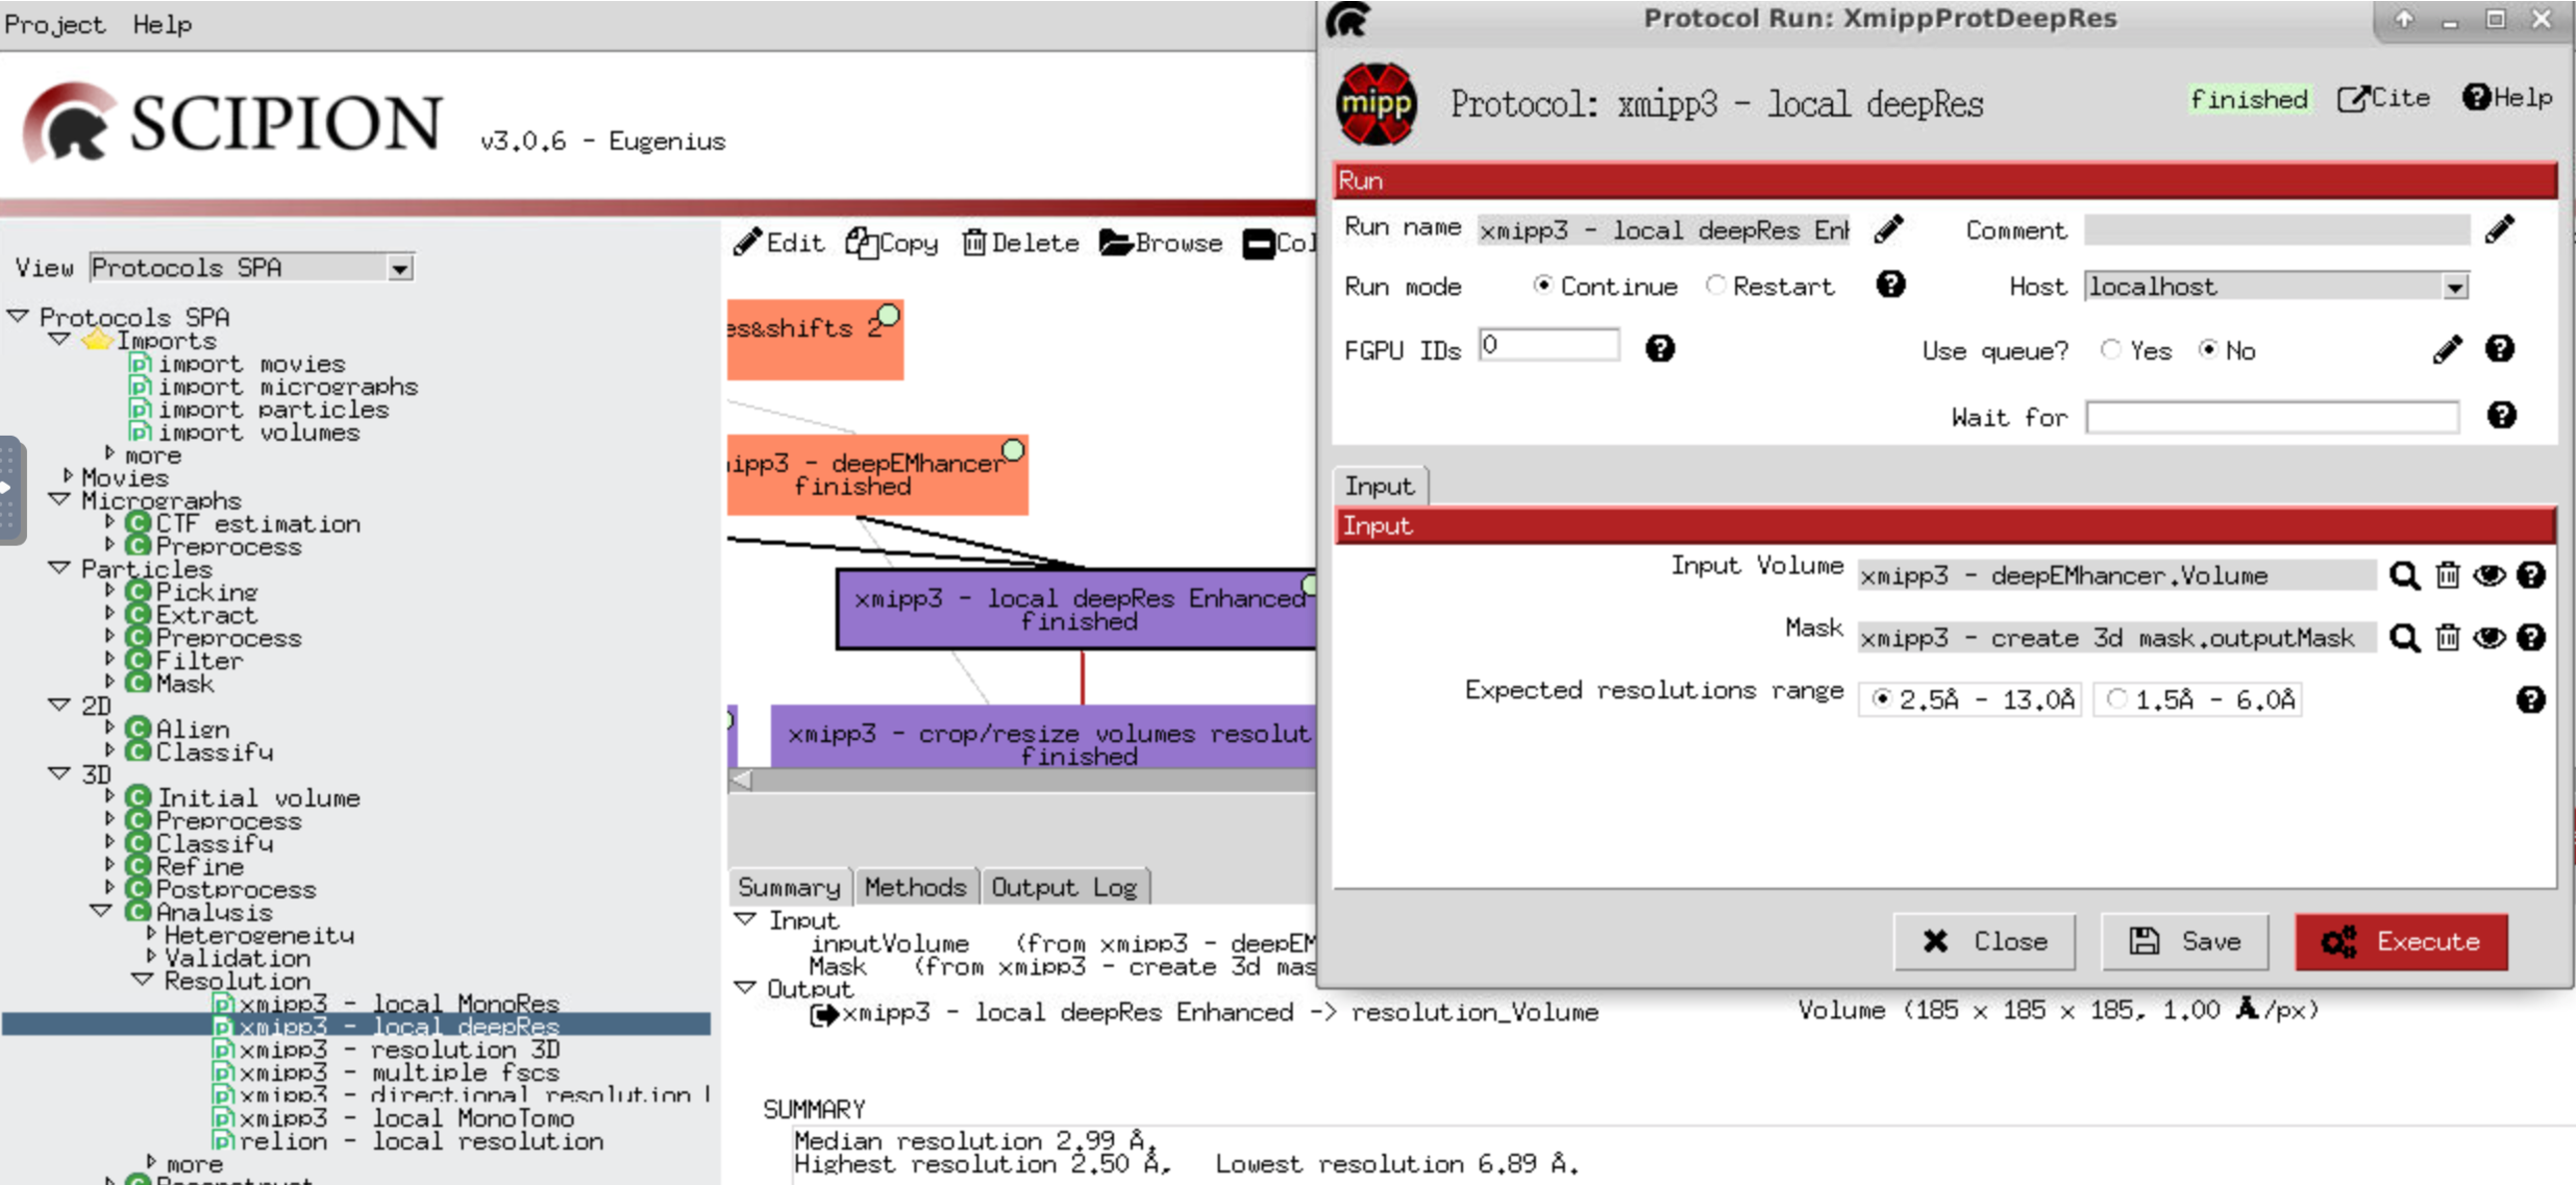
\includegraphics[width=0.95\textwidth]
  {{images/10g_xmipp3_localdeepRes2.pdf}}
  \caption{$Xmipp$ \ttt{local deepRes} Enhanced.}
  \label{fig:xmipp_localdeepRes2}
  \end{figure} 
  
   \begin{figure}[H]
  \centering
  \captionsetup{width=.8\linewidth} 
  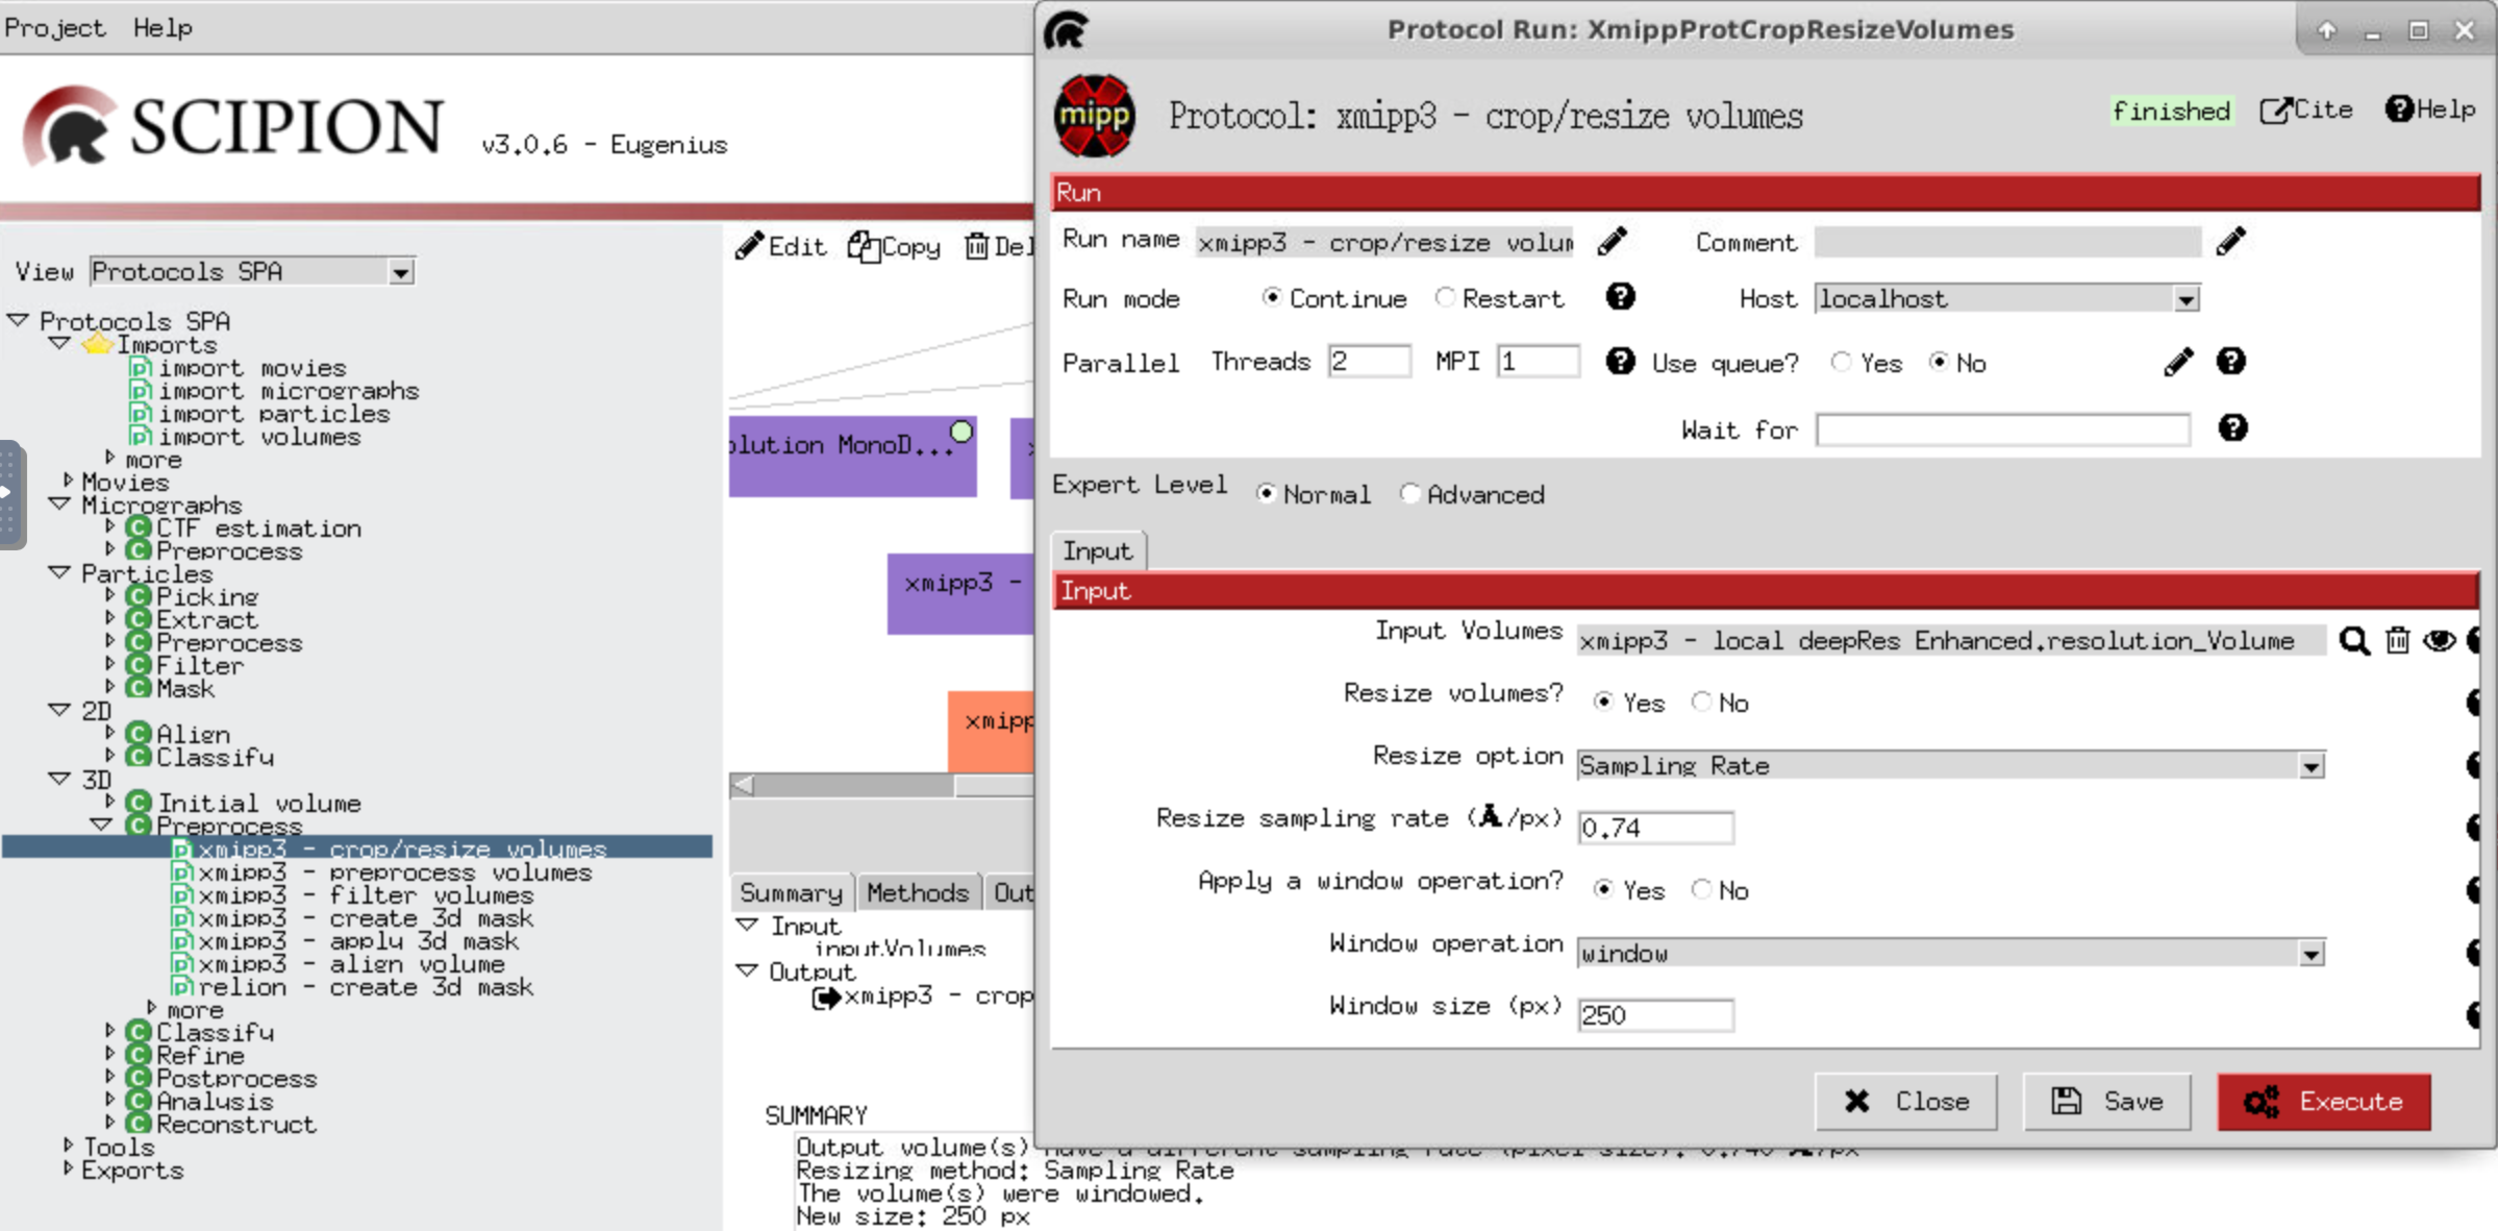
\includegraphics[width=0.95\textwidth]
  {{images/10i_xmipp3_cropresize2.pdf}}
  \caption{$Xmipp$ \ttt{crop/resize} volume resolution.}
  \label{fig:xmipp_croprs2}
  \end{figure} 
  
   \begin{figure}[H]
  \centering
  \captionsetup{width=.8\linewidth} 
  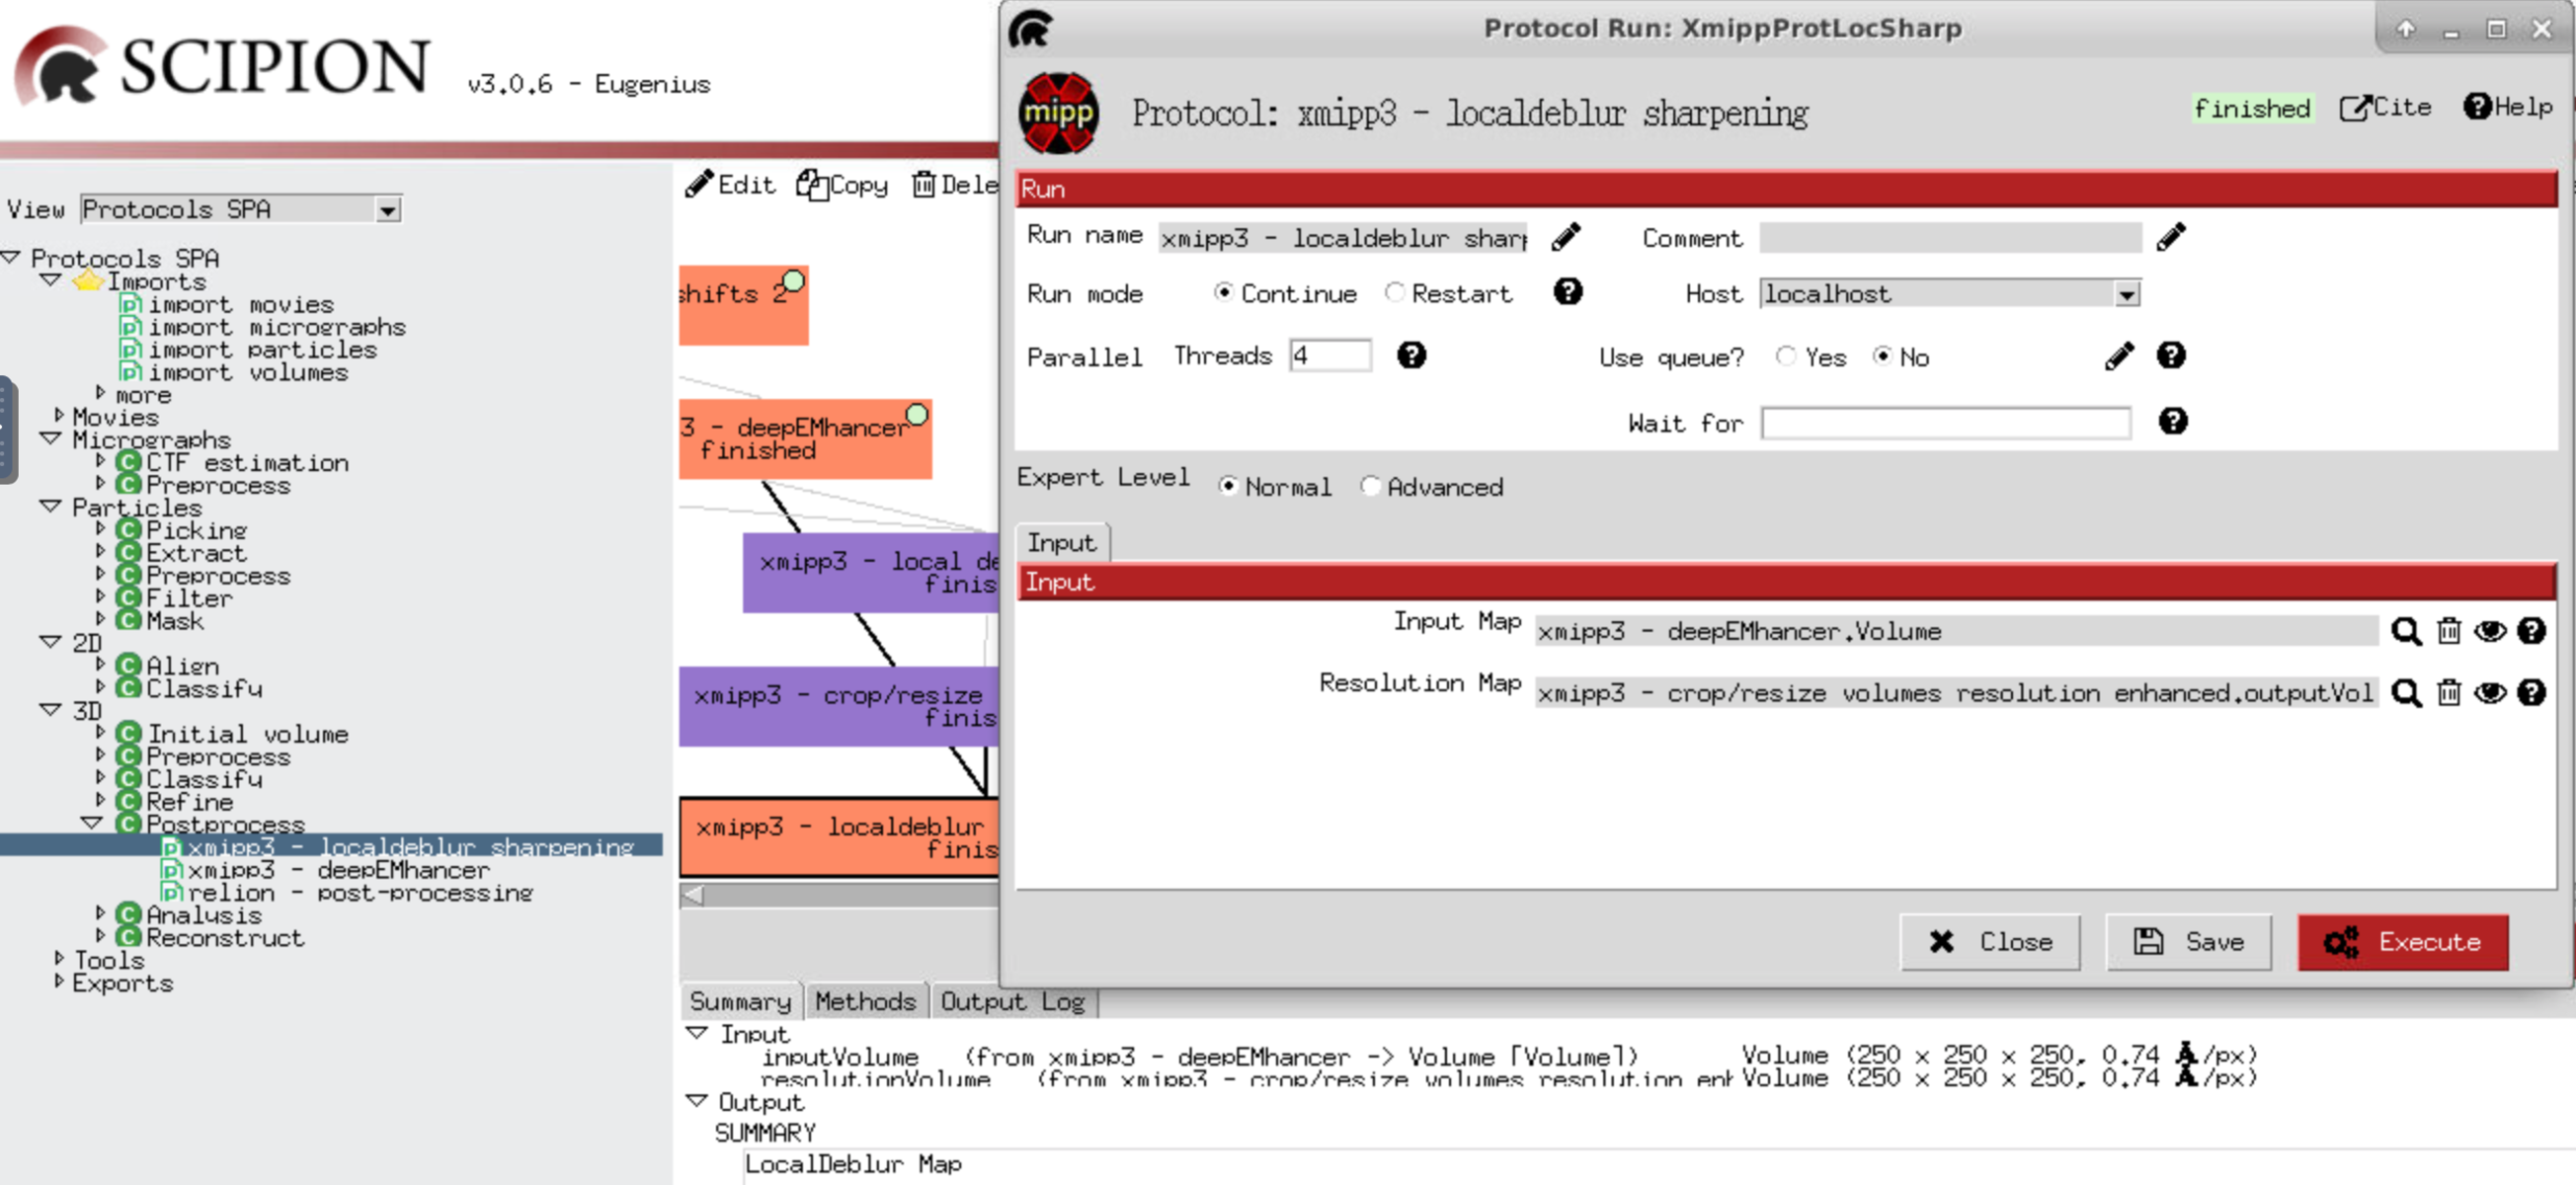
\includegraphics[width=0.95\textwidth]
  {{images/10k_xmipp3_localdeblur2.pdf}}
  \caption{$Xmipp$ \ttt{localdeblur sharpening}.}
  \label{fig:xmipp_localdeblur2}
  \end{figure} 
 
 After executing these protocols, we can observe that most of the results were improved, we increased the resolution and we obtained a further refined 3D structure. This tutorial is a good example that with good data we can reach high resolution in a short time.\\
 
   For more information: 
\begin{itemize}
   \item \textbf{Video tutorial}:  \url{https://www.youtube.com/watch?v=d2Lm2H0T7cc&list=PLQjWIcrmtc4JjyC-_BM99_XW-VsDa4_i3&index=30}.
   \item \textbf{Theoretical lecture}:  \url{https://www.youtube.com/watch?v=gglZdNEskJs&list=PLQjWIcrmtc4JjyC-_BM99_XW-VsDa4_i3&index=37}.
  \end{itemize}   
